\chapter[Theoretical Foundations: Convolution and the Fourier Basis]{Theoretical Foundations:\\Convolution and the Fourier Basis}

\section{Objective of This Section}

This section aims to reconstruct the theoretical reasoning proposed by
Tsuzuku and Sato~\cite{tsuzuku2019structural}. The aim is to understand why convolutional networks
are particularly sensitive to certain directions of the Fourier basis by mathematically characterizing
these vulnerabilities.

The general idea rests on the mathematical structure of convolutional layers.
To study this structure, we adopt a simplified linear framework, setting aside the components
commonly introduced into neural networks to break linearity
(such as nonlinear activation functions and \textit{max-pooling}).

The following developments use two standard linear algebra results:
the matrix representation of a linear map and the relationship between eigenvectors,
eigenvalues, and diagonalization. These results are reviewed in Appendices~\ref{app:representation-lineaire-matrice}
and~\ref{app:vecteurs-propres-diagonalisation}.

\section{Fourier and Vectorization Conventions}
\label{sec:conventions-fourier-vectorisation}

Before studying convolutions, we establish the conventions used throughout this chapter.

In what follows, all frequencies and spatial indices are interpreted modulo $N$.

\subsection{1D Fourier Basis and Discrete Transform}

For an integer $N \geq 1$, let
\[
    \mathbb{Z}_N = \{0,\dots,N-1\}
\]
denote the set of indices taken modulo $N$. In concrete terms, this means that index $N$ is identified
with index $0$, index $N+1$ with index $1$, and so on. This convention is used
throughout the chapter.

For each frequency $k\in\mathbb{Z}_N$, we define the normalized discrete Fourier vector
\begin{equation}
    \phi_k[n]
    =
    \frac{1}{\sqrt{N}}
    e^{2\pi i kn/N},
    \qquad n\in\mathbb{Z}_N.
    \label{eq:def_base_fourier_1d}
\end{equation}
The vector $\phi_k$ represents a discrete wave of frequency $k$. Small values of $k$
correspond to slow variations, while higher frequencies correspond to
faster oscillations over the $N$ signal points. The factor $1/\sqrt{N}$ normalizes the
vector, giving
\[
    \|\phi_k\|_2 = 1.
\]

We collect all these vectors in a single matrix:
\begin{equation}
    F_N
    =
    \begin{pmatrix}
    | & | &        & | \\
    \phi_0 & \phi_1 & \cdots & \phi_{N-1} \\
    | & | &        & |
    \end{pmatrix}.
    \label{eq:def_matrice_fourier_1d}
\end{equation}
The matrix $F_N$ therefore contains, column by column, all possible Fourier directions
for a signal of size $N$. With the chosen normalization, its columns form an
orthonormal basis of $\mathbb{C}^N$, that is,
\[
    F_N^H F_N = I_N,
    \qquad
    F_N^{-1}=F_N^H.
\]

The discrete Fourier transform then consists of expressing a signal
$x\in\mathbb{C}^N$ in this basis. Under our convention, the Fourier coefficients of $x$ are
given by
\begin{equation}
    \widehat{x}
    =
    F_N^H x,
\end{equation}
or, component by component,
\begin{equation}
    \widehat{x}[k]
    =
    \frac{1}{\sqrt{N}}
    \sum_{n=0}^{N-1}
    x[n]e^{-2\pi i kn/N}.
    \label{eq:def_dft_1d}
\end{equation}
The coefficient $\widehat{x}[k]$ measures the contribution of frequency $k$ to the signal.

Since $F_N$ is unitary, the signal can be reconstructed from its Fourier coefficients as
\begin{equation}
    x
    =
    F_N\widehat{x},
\end{equation}
or, component by component,
\begin{equation}
    x[n]
    =
    \frac{1}{\sqrt{N}}
    \sum_{k=0}^{N-1}
    \widehat{x}[k]e^{2\pi i kn/N}.
    \label{eq:def_idft_1d}
\end{equation}

\subsection{2D Fourier Basis}

We now move from 1D signals to 2D images. For an image
$X\in\mathbb{C}^{N\times N}$, we use spatial indices
\[
    (m,n)\in\mathbb{Z}_N^2.
\]
The index $m$ denotes the vertical position, and $n$ the horizontal position.

Similarly, a 2D frequency is described by a pair
\[
    (u,v)\in\mathbb{Z}_N^2.
\]
The index $u$ corresponds to the vertical frequency, while $v$ corresponds to the horizontal
frequency.

For each frequency pair $(u,v)$, we define the 2D Fourier image
\begin{equation}
    \Phi_{u,v}[m,n]
    =
    \phi_u[m]\phi_v[n]
    =
    \frac{1}{N}
    e^{2\pi i(um+vn)/N}.
    \label{eq:def_base_fourier_2d}
\end{equation}
This formula means that a 2D Fourier mode is obtained as the product of a vertical wave
and a horizontal wave, in matrix form: $\Phi_{u,v} = \phi_u \phi_v^T$.

Varying the frequencies $u$ and $v$ produces different periodic patterns in image
space. Visually, these patterns can take the form of stripes, grids, or oriented
oscillations whose density depends directly on the pair $(u,v)$. Adding a Fourier
direction to an image therefore amounts to superimposing a periodic geometric pattern.

\begin{figure}[H]
    \centering
    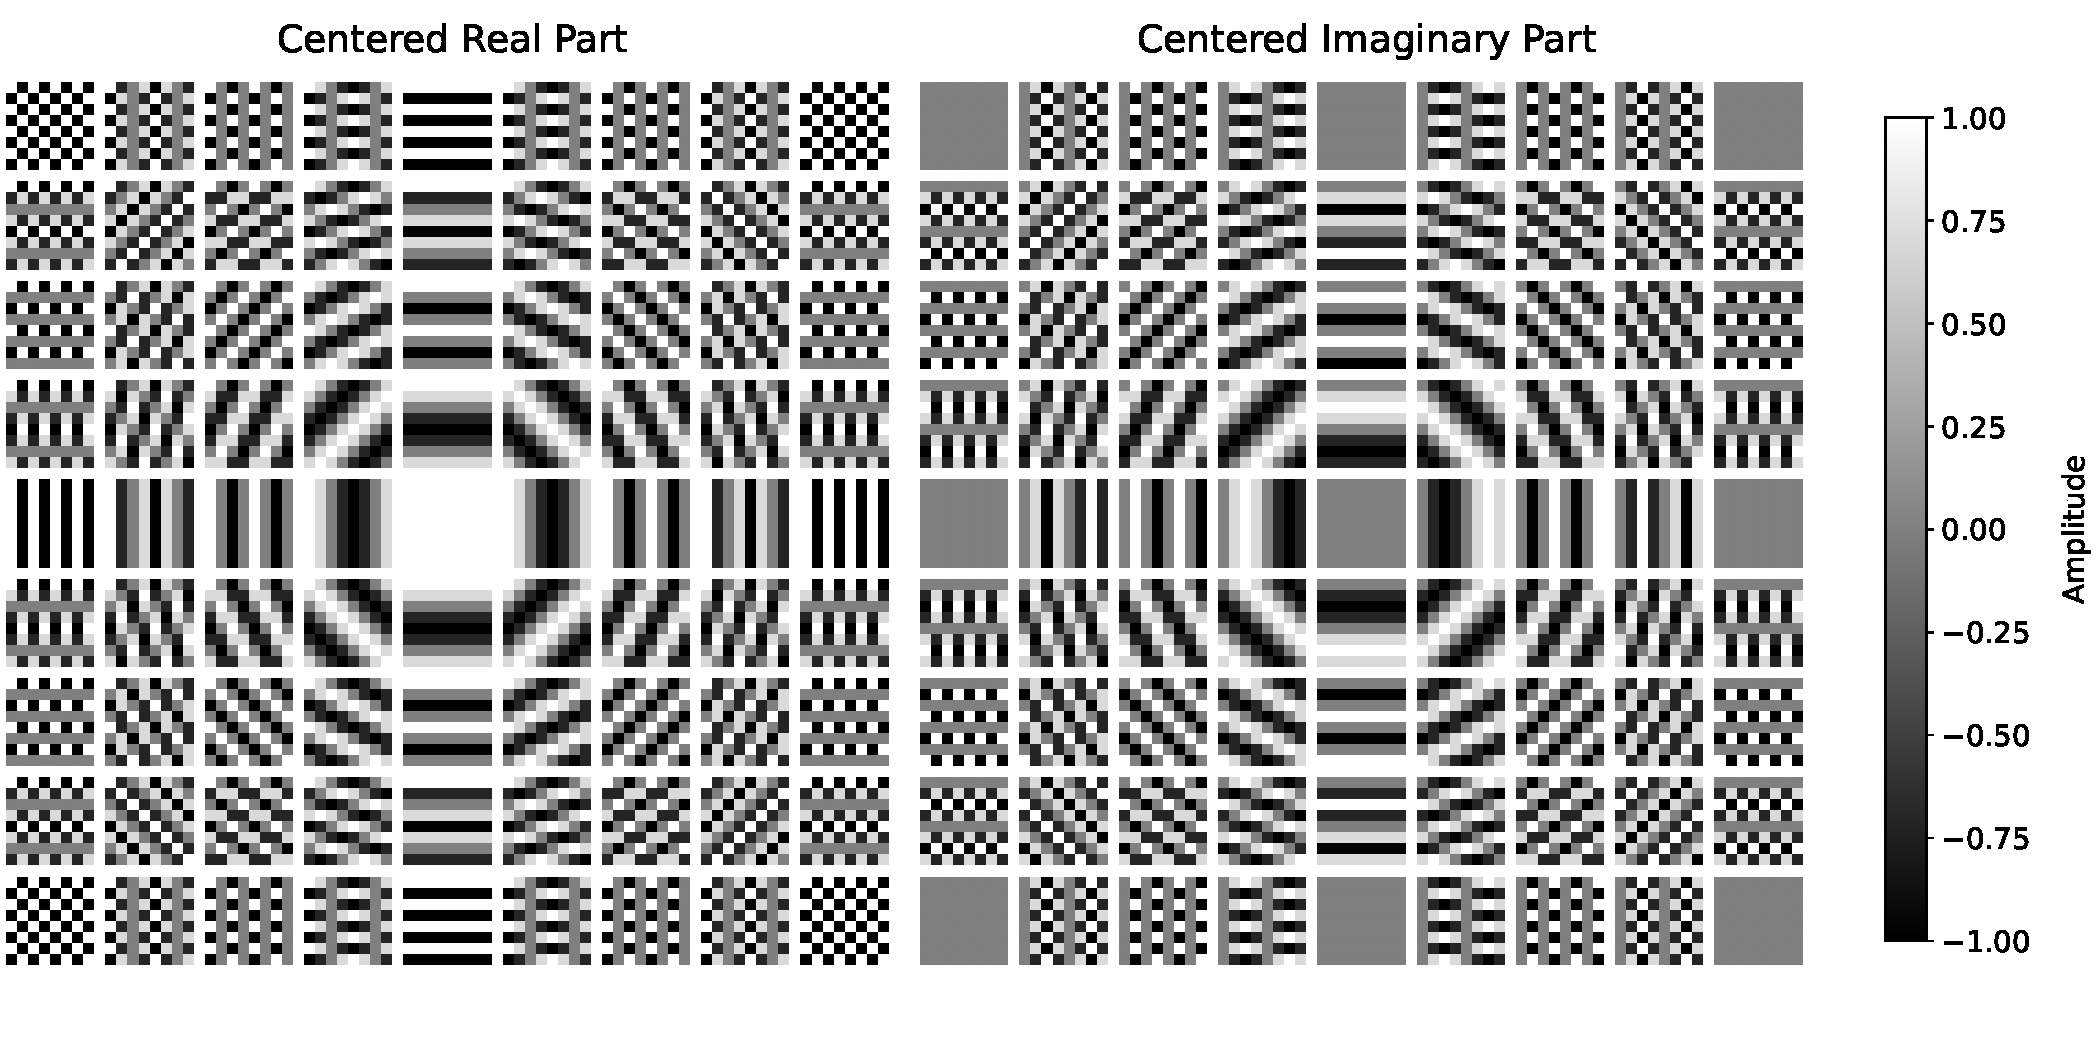
\includegraphics[width=0.95\textwidth]{figures/theory/fourier_basis_2d_en.pdf}
    \caption{Visualization of 2D Fourier basis functions for all frequency pairs $(u,v)$ of an image of size $9 \times 9$. The real and imaginary parts are displayed separately. Low frequencies lie at the center of the grids, while high frequencies lie at the edges.}
    \label{fig:fourier_basis_2d}
\end{figure}

In figures, frequencies are sometimes shown in a centered arrangement, with low frequencies
at the center of the image. This convention is convenient for visualization. In the formulas, however,
the indices always remain in $\{0,\dots,N-1\}$ and are interpreted modulo $N$.

\subsection{Vectorization and the Kronecker Product}

Throughout this chapter, we vectorize images by stacking their columns. For
$X\in\mathbb{C}^{N\times N}$, we therefore define
\begin{equation}
\operatorname{vec}(X)
=
\begin{pmatrix}
X[0,0] \\
X[1,0] \\
\vdots \\
X[N-1,0] \\
X[0,1] \\
\vdots \\
X[N-1,N-1]
\end{pmatrix}.
\label{eq:def_vectorisation_colonnes}
\end{equation}
The first column is read first, then the second, and so on. Under this convention,
entry $X[m,n]$ corresponds to the vectorized index
\[
    m+Nn.
\]

We also use the Kronecker product, denoted by $\otimes$. It is defined as follows: for
$A \in \mathbb{C}^{m \times n}$ and $B \in \mathbb{C}^{p \times q}$, the block matrix of size
$mp \times nq$ is defined by

$$
A \otimes B =
\begin{pmatrix}
a_{11}B & a_{12}B & \cdots & a_{1n}B \\
a_{21}B & a_{22}B & \cdots & a_{2n}B \\
\vdots  & \vdots  & \ddots & \vdots  \\
a_{m1}B & a_{m2}B & \cdots & a_{mn}B
\end{pmatrix}.
$$

In particular, it allows us to construct
a 2D Fourier basis from two 1D Fourier bases. The algebraic properties of
vectorization and the Kronecker product are established results in matrix analysis~\cite{horn2013matrix}.

Under our column-wise vectorization convention, in particular,
\begin{equation}
    \operatorname{vec}(ab^T)
    =
    b\otimes a.
    \label{eq:vec_produit_exterieur}
\end{equation}

Applying this identity to the Fourier image
\[
    \Phi_{u,v}=\phi_u\phi_v^T,
\]
gives
\begin{equation}
    \operatorname{vec}(\Phi_{u,v})
    =
    \phi_v\otimes\phi_u.
    \label{eq:vec_fourier_2d}
\end{equation}
Thus, throughout the remainder of the chapter, the column of $Q_N$ associated with the 2D frequency $(u,v)$ is denoted by
\[
    q_{u,v}
    =
    \phi_v\otimes\phi_u.
\]

We then denote by
\begin{equation}
    Q_N = F_N \otimes F_N
    \label{eq:def_base_fourier_2d_vectorisee}
\end{equation}
the vectorized 2D Fourier basis. Since $F_N$ is unitary,
\[
    Q_N^H Q_N = I_{N^2}.
\]
The columns of $Q_N$ form an orthonormal basis of $\mathbb{C}^{N^2}$.

With the preceding notation, the column associated with frequency $(u,v)$ is
\[
    (Q_N)_{w(u,v)}
    =
    q_{u,v}
    =
    \phi_v\otimes\phi_u.
\]
The index $w(u,v)$ is simply the flattened index that maps the frequency pair
$(u,v)$ to a single column index in $Q_N$. It is defined by
\begin{equation}
    w(u,v)=u+Nv.
    \label{eq:indice_frequence_aplati}
\end{equation}\

Conversely, given a flattened index $w\in\{0,\dots,N^2-1\}$, the corresponding frequency
pair is recovered as
\[
    u = w \bmod N,
    \qquad
    v = \left\lfloor \frac{w}{N} \right\rfloor.
\]

\section{Discrete Convolution in Dimension 1}

Before studying images, we begin with the simpler case of a periodic discrete signal represented
by one period $x = (x[0], x[1], \ldots, x[N-1])$ with $x[i] \in \mathbb{R}$.
Let $x \in \mathbb{R}^N$ be our signal and $h = (h[0], h[1], \ldots, h[N-1]) \in \mathbb{R}^N$ our filter (assumed
to have the same size as the signal, with zero-padding if necessary).
The circular convolution of $h$ and $x$ is defined as

\[
y[n] = (h * x)[n] = \sum_{k=0}^{N-1} h[k]\,x[(n-k) \bmod N] \text{~\cite{ImagerieNumeriqueTheme7Block2}}
\]

The modulo operation means that the signal indices are taken in
\(\mathbb{Z}_N\). 
Thus, when an index falls outside the interval \(\{0,\ldots,N-1\}\),
it is mapped back to its corresponding class in \(\mathbb{Z}_N\).
The signal is therefore interpreted as periodic, as illustrated in
Figure~\ref{fig:padding_circulaire}.

\begin{figure}[H]
    \centering
    \begin{tikzpicture}[
        node distance=0cm,
        cell/.style={rectangle, draw=black, thick, minimum width=1.2cm, minimum height=1.2cm, text centered, font=\large},
        pad/.style={rectangle, draw=gray, dashed, fill=gray!10, minimum width=1.2cm, minimum height=1.2cm, text centered, font=\large, text=gray}
    ]
    
    \node[cell] (x0) {$x_0$};
    \node[cell, right=of x0] (x1) {$x_1$};
    \node[cell, right=of x1] (x2) {$x_2$};
    \node[cell, right=of x2] (x3) {$x_3$};
    
    \node[pad, left=of x0] (pL1) {$x_3$};
    \node[pad, left=of pL1] (pL2) {$x_2$};
    
    \node[pad, right=of x3] (pR1) {$x_0$};
    \node[pad, right=of pR1] (pR2) {$x_1$};
    
    \draw [decorate,decoration={brace,amplitude=5pt,mirror}]
        (x0.south west) -- (x3.south east) node[midway,below=10pt] {Original signal $x$};
    
    \draw [decorate,decoration={brace,amplitude=5pt}, gray]
        (pL2.north west) -- (pL1.north east) node[midway,above=10pt] {\textit{Padding}};
        
    \draw [decorate,decoration={brace,amplitude=5pt}, gray]
        (pR1.north west) -- (pR2.north east) node[midway,above=10pt] {\textit{Padding}};

    \draw[->, thick, gray, dashed, bend left=45] (x3.north) to node[above] {} (pL1.north);
    \draw[->, thick, gray, dashed, bend right=45] (x0.south) to node[below] {} (pR1.south);

    \end{tikzpicture}
    \caption{Circular \textit{padding} for a 1D signal. The signal boundaries repeat periodically.}
    \label{fig:padding_circulaire}
\end{figure}

\paragraph{Remark on the periodicity assumption.}

In this section, we work with circular convolutions. This amounts to treating
signals as periodically extended: when we pass one end of the signal, we continue
from the other end. This assumption is mathematically useful because it allows
convolutions to be diagonalized by the discrete Fourier basis.

However, it does not always match the exact boundary behavior of real images:
if the ends do not join naturally, periodization can create an artificial
discontinuity. This point is discussed in greater detail in Appendix~\ref{app:periodicite-bords-gibbs}.

\section{Fourier Functions as Eigenfunctions of Circular Convolution}
\label{sec:fourier-vecteurs-propres}

\paragraph{One-dimensional case.}

We work in the space of periodic discrete signals with period $N$:
\[
V_N = \{x : \mathbb{Z}_N \rightarrow \mathbb{C}\}.
\]
An element of $V_N$ can be viewed either as a periodic discrete function or as a vector in $\mathbb{C}^N$.

For a fixed filter $h \in \mathbb{C}^N$, circular convolution defines a linear operator
\[
\mathcal{C}_h : V_N \rightarrow V_N,
\qquad
\mathcal{C}_h(x) = h * x.
\]

For each frequency $f \in \{0,\dots,N-1\}$, we use the normalized Fourier vector
$\phi_f$ defined in \eqref{eq:def_base_fourier_1d}.

The fundamental result connecting circular convolution and the Fourier basis is then

\begin{equation}
\mathcal{C}_h(\phi_f) = \lambda_f \phi_f,
\label{eq:fourier_fonction_propre_conv_1d}
\end{equation}

or, component by component,
\[
(h * \phi_f)[n] = \lambda_f \phi_f[n],
\]
where
\[
\lambda_f =
\sum_{k=0}^{N-1} h[k] e^{-2\mathrm{i}\pi f k/N}.
\]

Note that $\lambda_f$ depends on the filter $h$ and the frequency $f$,
but not on the position $n$. Thus, when the input to the circular convolution operator
is a Fourier mode, convolution does not alter its spatial form: it simply
multiplies it by a complex scalar. In other words, $\lambda_f$ is an eigenvalue and
$\phi_f$ an eigenfunction of the circular convolution operator
$\mathcal{C}_h$.

\begin{proof}
\begin{alignat*}{2}
    (\mathcal{C}_h(\phi_f))[n] &= (h * \phi_f)[n] \\
    &= \sum_{k=0}^{N-1} h[k]\,\phi_f[(n-k) \bmod N] \\
    \text{\small (periodicity of $\phi_f$)} \quad &= \sum_{k=0}^{N-1} h[k]\,\phi_f[n-k] \\
    \text{\small (property of exponentials)} \quad &= \sum_{k=0}^{N-1} h[k] e^{-2\mathrm{i}\pi f k/N}\phi_f[n] \\
    &= \left(\sum_{k=0}^{N-1} h[k] e^{-2\mathrm{i}\pi f k/N}\right)\phi_f[n] \\
    &= \lambda_f \phi_f[n].
\end{alignat*}

\end{proof}

This result corresponds to the discrete convolution theorem: in the Fourier domain,
circular convolution becomes frequency-wise multiplication. Thus,
when the input is a pure Fourier mode \(\phi_f\), convolution does not change
its frequency; it only multiplies it by a scalar. We therefore obtain Equation~\ref{eq:fourier_fonction_propre_conv_1d}.

\subsection{Consequence: Diagonalization of Circulant Matrices}

For a fixed filter $h$, 1D circular convolution defines a linear map $\mathbb{C}^N \rightarrow \mathbb{C}^N$,
since for all $x, y \in \mathbb{C}^N$ and all $\alpha, \beta \in \mathbb{C}$,
\begin{align*}
h * (\alpha x + \beta y) &= \alpha (h * x) + \beta (h * y)
\end{align*}

\begin{proof}
\begin{alignat*}{2}
    (h * (\alpha x + \beta y))[n] &= \sum_{k=0}^{N-1} h[k]\,(\alpha x + \beta y)[(n-k) \bmod N]  \\
    &= \sum_{k=0}^{N-1} h[k]\,(\alpha x[(n-k) \bmod N] + \beta y[(n-k) \bmod N])  \\
    &= \alpha \sum_{k=0}^{N-1} h[k]\,x[(n-k) \bmod N] + \beta \sum_{k=0}^{N-1} h[k]\,y[(n-k) \bmod N]  \\
    &= \alpha (h * x)[n] + \beta (h * y)[n].
\end{alignat*}

\end{proof}

Since this operation is linear, the result reviewed in Appendix~\ref{app:representation-lineaire-matrice}
guarantees that, once a basis has been chosen, it can be represented by a matrix
$C_h \in \mathbb{C}^{N \times N}$ such that, for every input signal $x \in \mathbb{C}^N$,

$$
y = C_h x.
$$

Here, $C_h$ is a circulant matrix constructed from the filter $h$. Its first row is arranged to reproduce $y[0]$,
and each subsequent row is obtained by a circular shift:

$$
C_h =
\begin{pmatrix}
h[0] & h[N-1] & h[N-2] & \cdots & h[1] \\
h[1] & h[0] & h[N-1] & \cdots & h[2] \\
h[2] & h[1] & h[0] & \cdots & h[3] \\
\vdots & \vdots & \vdots & \ddots & \vdots \\
h[N-1] & h[N-2] & h[N-3] & \cdots & h[0]
\end{pmatrix}.
$$

Indeed, $y[0] = h[0]x[0] + h[1]x[N-1] + \cdots + h[N-1]x[1]$ is the first row of $C_h$
multiplied by the vector $x$. Applying the same reasoning iteratively gives the other elements of $y$.

\vspace{0.5cm}

In the standard basis of $\mathbb{C}^N$, the linear operator $\mathcal{C}_h$
is represented by the circulant matrix $C_h$. The relation
$\mathcal{C}_h(\phi_f) = \lambda_f \phi_f$ can then be rewritten in matrix form:

\begin{equation}
    C_h \phi_f = \lambda_f \phi_f
    \label{eq:fourier_eigen_matrice}
\end{equation}

Thus, each Fourier function $\phi_f$ is an eigenvector of the circulant matrix $C_h$,
with associated eigenvalue $\lambda_f$. This means that, in the circular
setting, convolution acts diagonally in the Fourier basis.

Using the Fourier matrix $F_N$ defined in \eqref{eq:def_matrice_fourier_1d},
we collect the eigenvalues in the diagonal matrix
$$
\Lambda_h =
\operatorname{diag}(\lambda_0,\lambda_1,\ldots,\lambda_{N-1}).
$$

Combining the vector equalities \eqref{eq:fourier_eigen_matrice} for all frequencies gives

\begin{align}
C_h F_N &= F_N \Lambda_h \notag \\
\text{(by unitarity of \(F_N\))}\qquad
\Longleftrightarrow\quad
C_h &= F_N \Lambda_h F_N^H.
\end{align}

\section{Circular Convolution in Dimension 2}
\label{sec:convolution-circulaire-2d}

We now extend the preceding result to square images. Let
$X\in\mathbb{C}^{N\times N}$ be an image and
$h\in\mathbb{C}^{N\times N}$ a filter. 2D circular convolution is defined by
\begin{equation}
    Y[m,n]
    =
    (h * X)[m,n]
    =
    \sum_{a=0}^{N-1}
    \sum_{b=0}^{N-1}
    h[a,b]\,
    X[(m-a)\bmod N,\,(n-b)\bmod N].
    \label{eq:def_convolution_circulaire_2d}
\end{equation}

We use the 2D Fourier images defined in \eqref{eq:def_base_fourier_2d}:
\[
    \Phi_{u,v}[m,n]
    =
    \phi_u[m]\phi_v[n].
\]
As in dimension 1, a circular shift of a Fourier basis function does not change its form, but
multiplies it by a complex factor:
\[
    \phi_u[(m-a)\bmod N]
    =
    e^{-2\pi iua/N}\phi_u[m],
    \qquad
    \phi_v[(n-b)\bmod N]
    =
    e^{-2\pi ivb/N}\phi_v[n].
\]
Thus,
\[
    \Phi_{u,v}[(m-a)\bmod N,(n-b)\bmod N]
    =
    e^{-2\pi i(ua+vb)/N}
    \Phi_{u,v}[m,n],
\]

where $(ua + vb) \in \mathbb{Z}_N$.

Applying 2D circular convolution to $\Phi_{u,v}$ gives
\begin{align}
(h * \Phi_{u,v})[m,n]
&=
\sum_{a=0}^{N-1}
\sum_{b=0}^{N-1}
h[a,b]\,
\Phi_{u,v}[(m-a)\bmod N,(n-b)\bmod N]
\nonumber \\
&=
\left(
\sum_{a=0}^{N-1}
\sum_{b=0}^{N-1}
h[a,b]e^{-2\pi i(ua+vb)/N}
\right)
\Phi_{u,v}[m,n].
\end{align}

We therefore define
\begin{equation}
    \lambda_{u,v}
    =
    \sum_{a=0}^{N-1}
    \sum_{b=0}^{N-1}
    h[a,b]e^{-2\pi i(ua+vb)/N}.
    \label{eq:valeur_propre_convolution_2d}
\end{equation}
Finally, we obtain
\begin{equation}
    h * \Phi_{u,v}
    =
    \lambda_{u,v}\Phi_{u,v}.
    \label{eq:fourier_fonction_propre_conv_2d}
\end{equation}

\section{Matrix Representation of a 2D Convolution}

We now use the column-wise vectorization defined in
\eqref{eq:def_vectorisation_colonnes}. Since circular convolution is linear, there exists
a matrix
\[
    M \in \mathbb{C}^{N^2\times N^2}
\]
such that
\begin{equation}
    \operatorname{vec}(Y)
    =
    M\operatorname{vec}(X).
\end{equation}

In other words, the coefficient of $M$ at row $m+Nn$ and column $r+Ns$ indicates how pixel
$X[r,s]$ contributes to pixel $Y[m,n]$.

The matrix $M$ applies the filter $h$ to every pixel of our image $X$ in a single operation.
To do so, $M$ has a block-circulant structure with circulant blocks (BCCB),
as illustrated below:

\begin{figure}[H]
\centering

\begin{tikzpicture}[
    scale=0.75, transform shape, % Réduction globale équilibrée
    font=\small,
    block/.style={
        draw=black!65,
        rounded corners=1pt,
        minimum width=1.0cm,  % Réduit de 1.25
        minimum height=0.55cm, % Réduit de 0.70
        inner sep=1pt,
        fill=gray!6,
        align=center
    },
    diagblock/.style={
        block,
        fill=gray!18,
        draw=black!85,
        line width=0.5pt
    },
    frame/.style={
        draw=black!85,
        rounded corners=2pt,
        line width=0.6pt
    },
    arrow/.style={
        -{Stealth[length=1.5mm]},
        semithick,
        black!65
    }
]

% --- Matrice M (plus compacte) ---
\matrix (B) [
    matrix of nodes,
    nodes={block},
    row sep=1.5pt,    % Espacement réduit
    column sep=1.5pt  % Espacement réduit
] {
|[diagblock]|$C_0$     & $C_{N-1}$ & $\cdots$ & $C_2$     & $C_1$     \\
$C_1$                 & |[diagblock]|$C_0$ & $\cdots$ & $C_3$     & $C_2$     \\
$\vdots$              & $\vdots$   & $\ddots$ & $\vdots$  & $\vdots$  \\
$C_{N-2}$             & $C_{N-3}$  & $\cdots$ & |[diagblock]|$C_0$ & $C_{N-1}$ \\
$C_{N-1}$             & $C_{N-2}$  & $\cdots$ & $C_1$     & |[diagblock]|$C_0$ \\
};

\node[frame, fit=(B-1-1)(B-5-5), inner sep=3pt] (bigmatrix) {};

% Titre compact avec sous-titre intégré
\node[above=2pt of bigmatrix, align=center] {
    \textbf{\(M \in\mathbb{C}^{N^2\times N^2}\)} \\ 
    \scriptsize (Block-circulant: shifts of blocks)
};

% --- Flèche de zoom plus courte ---
\draw[arrow] (bigmatrix.east) -- ++(0.7,0) node[midway, above, font=\tiny] {zoom};

% --- Bloc Ck (Matrice resserrée) ---
\node[anchor=west] (circulant) at ($(bigmatrix.east)+(0.9cm,0)$) {$\displaystyle
C_k =
\begin{bmatrix}
h_{0,k}     & \cdots & h_{1,k} \\
h_{1,k}     & \cdots & h_{2,k} \\
\vdots      & \ddots & \vdots  \\
h_{N-1,k}   & \cdots & h_{0,k}
\end{bmatrix}
$};

\node[frame, fit=(circulant), inner sep=2pt] (smallmatrix) {};

% Titre compact pour Ck
\node[above=2pt of smallmatrix, align=center] {
    \textbf{Circulant block \(C_k\)} \\
    \scriptsize (internal shifts)
};

\end{tikzpicture}

\caption{Compact structure of a BCCB (doubly circulant) matrix.}
\label{fig:bccb-structure}
\end{figure}

We therefore call $M$ a \textbf{BCCB} matrix (\textit{Block-Circulant with Circulant Blocks}~\cite{jain1989fundamentals}).
Details are provided in Appendix~\ref{app:preuve_bccb}.

The spectral result obtained for 2D circular convolution then becomes, in vectorized form,
\[
    M\operatorname{vec}(\Phi_{u,v})
    =
    \lambda_{u,v}\operatorname{vec}(\Phi_{u,v}).
\]

\subsection{Diagonalization by the Kronecker Product of Fourier Bases}

From the preceding result \ref{eq:fourier_fonction_propre_conv_2d}, since \(q_{u,v}=\operatorname{vec}(\Phi_{u,v})\), we obtain
\[
    M q_{u,v}
    =
    \lambda_{u,v} q_{u,v}.
\]
Combining the equalities for all frequencies gives the matrix identity
\begin{equation}
    \begin{split}
        M Q_N &= Q_N \Lambda_h \\
        \Longleftrightarrow \text{\footnotesize (unitarity of $Q_N$)} \quad M &= Q_N \Lambda_h Q_N^H.
    \end{split}
    \label{eq:diagonalisation_conv_2d}
\end{equation}
Here, $\Lambda_h$ is the diagonal matrix containing the eigenvalues $\lambda_{u,v}$
in the same order as the columns $q_{u,v}$ of $Q_N$.

\section{Extension to the Multichannel Case}

So far, we have considered single-channel convolution, where the input
and output images each have a single channel (for example, a grayscale image).
We now consider the more general case of multichannel convolution:
\[
    X \in\mathbb{C}^{m_{in} \times N \times N}, \qquad Y \in\mathbb{C}^{m_{out} \times N \times N},
\]
where $m_{in}$ and $m_{out}$ denote the number of input and output channels, respectively.

For each output channel $Y_i$,
\begin{equation}
    Y_i = \sum_{j=1}^{m_{in}} h_{i,j} * X_j \qquad\text{for } i=1,\dots,m_{out},
    \label{eq:conv_multi}
\end{equation}
where $h_{i,j}$ is the convolution filter applied to input channel $j$ to produce output channel $i$.

% \begin{figure}[H]
%     \centering
%     % J'ai baissé très légèrement le scale à 0.85 pour que ce schéma plus large rentre 
%     % parfaitement dans les marges classiques d'un document A4.
%     \begin{tikzpicture}[>=stealth, font=\sffamily, scale=0.85, every node/.style={transform shape}]
        
%         % ==========================================
%         % Couleurs
%         % ==========================================
%         \definecolor{gridblue}{HTML}{006699}
%         \definecolor{gridred}{HTML}{E74C3C}
%         \definecolor{gridteal}{HTML}{148F77}
%         \definecolor{gridorange}{HTML}{F39C12}
%         \definecolor{bglight}{HTML}{F8F9FA}

%         % ==========================================
%         % Zones de fond (Structuration élargie)
%         % ==========================================
%         \draw[fill=bglight, draw=gray!40, dashed, rounded corners=5pt] 
%             (-1.0, -1.0) rectangle (1.0, 6.0);
%         \node[gray, font=\bfseries\small] at (0, 5.65) {Entrée $X$};

%         \draw[fill=bglight, draw=gray!40, dashed, rounded corners=5pt] 
%             (3.0, -1.0) rectangle (5.0, 6.0);
%         \node[gray, font=\bfseries\small, align=center] at (4.0, 5.65) {Filtres $h_i$};

%         \draw[fill=bglight, draw=gray!40, dashed, rounded corners=5pt] 
%             (7.0, -1.0) rectangle (9.0, 6.0);
%         \node[gray, font=\bfseries\small, align=center] at (8.0, 5.65) {Cartes $Z_i$};

%         \draw[fill=bglight, draw=gray!40, dashed, rounded corners=5pt] 
%             (10.8, -1.0) rectangle (15.5, 6.0);
%         \node[gray, font=\bfseries\small, align=center] at (13.15, 5.65) {Somme et Sortie};

%         % ==========================================
%         % 1. Canal Supérieur (m_in)
%         % ==========================================
%         % X_min (Centre x=0, y=3.8)
%         \filldraw[fill=gridblue!10, draw=gridblue, thick] 
%             (-0.625, 3.175) rectangle ++(1.25,1.25);
%         \draw[gridblue!40, step=0.3125] (-0.625, 3.175) grid ++(1.25,1.25);
%         \node[gridblue, font=\bfseries\scriptsize, fill=white, fill opacity=0.8, text opacity=1, inner sep=1.5pt] 
%             at (0, 3.8) {$X_{m_{\mathrm{in}}}$};

%         % Conv node * (Centre x=4.0, y=3.8)
%         \node[circle, draw=gridorange, fill=gridorange!10, thick, minimum size=0.5cm, inner sep=0pt] 
%             (convtop) at (4.0, 3.8) {$*$};

%         % h_min (Centre x=4.0, y=5.0)
%         \filldraw[fill=gridred!10, draw=gridred, thick] 
%             (3.575, 4.575) rectangle ++(0.85,0.85);
%         \draw[gridred!45, step=0.2125] (3.575, 4.575) grid ++(0.85,0.85);
%         \node[gridred, font=\bfseries\scriptsize, fill=white, fill opacity=0.8, text opacity=1, inner sep=1.5pt] 
%             at (4.0, 5.0) {$h_{i,m_{\mathrm{in}}}$};

%         % Z_min (Centre x=8.0, y=3.8)
%         \filldraw[fill=gridorange!15, draw=gridorange, thick] 
%             (7.45, 3.25) rectangle ++(1.10,1.10);
%         \draw[gridorange!45, step=0.275] (7.45, 3.25) grid ++(1.10,1.10);
%         \node[gridorange!80!black, font=\bfseries\scriptsize, fill=white, fill opacity=0.8, text opacity=1, inner sep=1.5pt] 
%             at (8.0, 3.8) {$Z_{i,m_{\mathrm{in}}}$};

%         % Flèches Canal m_in
%         \draw[->, thick, gridblue] (0.625, 3.8) -- (convtop.west);
%         \draw[->, thick, gridred] (4.0, 4.575) -- (convtop.north);
%         \draw[->, thick, gridorange] (convtop.east) -- (7.45, 3.8);

%         % ==========================================
%         % 2. Canal Inférieur (1)
%         % ==========================================
%         % X_1 (Centre x=0, y=0)
%         \filldraw[fill=gridblue!25, draw=gridblue, thick] 
%             (-0.625, -0.625) rectangle ++(1.25,1.25);
%         \draw[gridblue!45, step=0.3125] (-0.625, -0.625) grid ++(1.25,1.25);
%         \node[gridblue, font=\bfseries\scriptsize, fill=white, fill opacity=0.85, text opacity=1, inner sep=2pt] 
%             at (0, 0) {$X_1$};

%         % Conv node * (Centre x=4.0, y=0)
%         \node[circle, draw=gridorange, fill=gridorange!10, thick, minimum size=0.5cm, inner sep=0pt] 
%             (convbot) at (4.0, 0) {$*$};

%         % h_1 (Centre x=4.0, y=1.2)
%         \filldraw[fill=gridred!25, draw=gridred, thick] 
%             (3.575, 0.775) rectangle ++(0.85,0.85);
%         \draw[gridred!45, step=0.2125] (3.575, 0.775) grid ++(0.85,0.85);
%         \node[gridred, font=\bfseries\scriptsize, fill=white, fill opacity=0.85, text opacity=1, inner sep=2pt] 
%             at (4.0, 1.2) {$h_{i,1}$};

%         % Z_1 (Centre x=8.0, y=0)
%         \filldraw[fill=gridorange!25, draw=gridorange, thick] 
%             (7.45, -0.55) rectangle ++(1.10,1.10);
%         \draw[gridorange!45, step=0.275] (7.45, -0.55) grid ++(1.10,1.10);
%         \node[gridorange!80!black, font=\bfseries\scriptsize, fill=white, fill opacity=0.85, text opacity=1, inner sep=2pt] 
%             at (8.0, 0) {$Z_{i,1}$};

%         % Flèches Canal 1
%         \draw[->, thick, gridblue] (0.625, 0) -- (convbot.west);
%         \draw[->, thick, gridred] (4.0, 0.775) -- (convbot.north);
%         \draw[->, thick, gridorange] (convbot.east) -- (7.45, 0);

%         % ==========================================
%         % 3. Intermédiaires (Points de suspension)
%         % ==========================================
%         \node[gridblue, font=\Large] at (0, 1.9) {$\vdots$};
%         \node[gridorange, font=\Large] at (4.0, 1.9) {$\vdots$}; 
%         \node[gridorange!80!black, font=\Large] at (8.0, 1.9) {$\vdots$};

%         % ==========================================
%         % 4. Somme & Sortie
%         % ==========================================
%         % Sum (Centre x=12.0)
%         \node[circle, draw=gridteal, fill=gridteal!10, thick, minimum size=0.85cm] 
%             (sum) at (12.0, 1.9) {\Large $\sum$};
%         \node[gridteal, font=\scriptsize, align=center] at (12.0, 1.1) {somme\\sur $j$};

%         % Flèches Z -> Somme
%         \draw[->, thick, gridorange] (8.55, 3.8) to[out=0,in=135] (sum.north west);
%         \draw[->, thick, gridorange] (8.55, 0) to[out=0,in=225] (sum.south west);

%         % Y_i (Centre x=14.2)
%         \filldraw[fill=gridteal!22, draw=gridteal, thick] 
%             (13.525, 1.225) rectangle ++(1.35,1.35);
%         \draw[gridteal!45, step=0.3375] (13.525, 1.225) grid ++(1.35,1.35);
%         \node[gridteal, font=\bfseries\scriptsize, fill=white, fill opacity=0.85, text opacity=1, inner sep=2pt] 
%             at (14.2, 1.9) {$Y_i$};

%         % Flèche Somme -> Y_i
%         \draw[->, thick, gridteal] (sum.east) -- (13.525, 1.9);

%         % ==========================================
%         % 5. Equations Mathématiques (En bas, aérées)
%         % ==========================================
%         \node[gridblue, font=\bfseries\small] at (0, -1.8) {$X \in \mathbb{C}^{m_{\mathrm{in}}\times N\times N}$};
%         \node[gridred, font=\bfseries\small] at (4.0, -1.8) {$h_i \in \mathbb{C}^{m_{\mathrm{in}}\times k\times k}$};
%         \node[gridorange!80!black, font=\bfseries\small] at (8.0, -1.8) {$Z_{i,j}=h_{i,j} * X_j$};
%         \node[gridteal, font=\bfseries\small] at (13.15, -1.8) {$Y_i=\displaystyle\sum_{j=1}^{m_{\mathrm{in}}} Z_{i,j}$};

%     \end{tikzpicture}

%     \vspace{0.3cm}
%     \caption{
%     Convolution multi-canaux produisant un canal de sortie $Y_i$.
%     }
%     \label{fig:conv_multi_canaux}
% \end{figure}

\subsection{Channel Mixing at a Fixed Frequency}
\label{subsec:melange_canaux_frequence_fixee}

Consider a spatial frequency $(u,v)$ and the corresponding Fourier image $\Phi_{u,v}$.
Assume that each input channel contains this same spatial frequency, but with a different
amplitude:
\[
    X_j = \alpha_j \Phi_{u,v},
    \qquad j=1,\dots,m_{\mathrm{in}}.
\]
The vector
\[
    \alpha = (\alpha_1,\dots,\alpha_{m_{\mathrm{in}}})^T
\]
therefore contains the amplitudes of this frequency in the different input channels.

Substituting these inputs into \eqref{eq:conv_multi} and using linearity of convolution gives, for output channel $i$,
\begin{align*}
Y_i
&=
\sum_{j=1}^{m_{\mathrm{in}}} h_{i,j} * X_j \\
&=
\sum_{j=1}^{m_{\mathrm{in}}} \alpha_j (h_{i,j} * \Phi_{u,v}) \\
&=
\sum_{j=1}^{m_{\mathrm{in}}} \alpha_j \lambda^{i,j}_{u,v}\Phi_{u,v} \\
&=
\left(
    \sum_{j=1}^{m_{\mathrm{in}}}
    \lambda^{i,j}_{u,v}\alpha_j
\right)
\Phi_{u,v}.
\end{align*}

We then introduce the mixing matrix associated with frequency $(u,v)$:
\[
    G^{(u,v)} \in \mathbb{C}^{m_{\mathrm{out}}\times m_{\mathrm{in}}},
    \qquad
    G^{(u,v)}_{i,j}
    =
    \lambda^{i,j}_{u,v}.
\]
If $\beta\in\mathbb{C}^{m_{\mathrm{out}}}$ denotes the output amplitudes of this same frequency,
we can simply write
\[
    \beta = G^{(u,v)}\alpha.
\]

This expression summarizes the role of multichannel convolution: for a fixed spatial frequency,
it performs linear mixing across channels.

\subsection{Global Matrix Form}

To express the multichannel operation in global matrix form, we define
\[
\mathbf{x}
=
\begin{pmatrix}
\operatorname{vec}(X_1) \\
\vdots \\
\operatorname{vec}(X_{m_{\mathrm{in}}})
\end{pmatrix}
\in \mathbb{C}^{m_{\mathrm{in}}N^2},
\qquad
\mathbf{y}
=
\begin{pmatrix}
\operatorname{vec}(Y_1) \\
\vdots \\
\operatorname{vec}(Y_{m_{\mathrm{out}}})
\end{pmatrix}
\in \mathbb{C}^{m_{\mathrm{out}}N^2}.
\]

For each channel pair $(i,j)$, let $B^{i,j}$ denote the spatial convolution matrix
associated with filter $h_{i,j}$, that is, the matrix applying convolution between input
channel $j$ and output channel $i$.
We use the vectorized 2D Fourier basis $Q_N$ defined in
\eqref{eq:def_base_fourier_2d_vectorisee}. For each channel pair $(i,j)$, the matrix
$B^{i,j}$ can therefore be diagonalized as
\[
    B^{i,j}
    =
    Q_N D^{i,j} Q_N^H,
\]
where
\[
D^{i,j}
=
\operatorname{diag}\bigl(
\lambda^{i,j}_{u,v}
\bigr)_{(u,v)\in\{0,\dots,N-1\}^2}.
\]

The diagonal entries of $D^{i,j}$ are ordered according to the flattened index
$w(u,v)$ defined in \eqref{eq:indice_frequence_aplati}.

We can now introduce the global matrix $M \in \mathbb{C}^{m_{out}N^2 \times m_{in}N^2}$,
which represents the entire convolutional layer as a block matrix of size
$m_{out} \times m_{in}$, where each block $(i,j)$ corresponds to the application of filter $h_{i,j}$:

$$
M =
\begin{pmatrix}
B^{1,1} & \cdots & B^{1,m_{in}} \\
\vdots & \ddots & \vdots \\
B^{m_{out},1} & \cdots & B^{m_{out},m_{in}}
\end{pmatrix}.
$$

Since the same basis $Q_N$ diagonalizes all spatial blocks $B^{i,j}$, we can factor out the spatial
change of basis on either side of the block matrix. This gives

\begin{equation}
    M = (I_{m_{out}} \otimes Q_N) L (I_{m_{in}} \otimes Q_N)^H
    \label{eq:factorisation_M}
\end{equation}

where $L \in \mathbb{C}^{m_{out}N^2 \times m_{in}N^2}$ is a block matrix with diagonal blocks:

$$
L =
\begin{pmatrix}
D^{1,1} & \cdots & D^{1,m_{in}} \\
\vdots & \ddots & \vdots \\
D^{m_{out},1} & \cdots & D^{m_{out},m_{in}}
\end{pmatrix}.
$$

\vspace{0.5cm}
\begin{proof}

By the definition of the Kronecker product, the operations
$I_{m_{out}} \otimes Q_N$ and $(I_{m_{in}} \otimes Q_N)^H = I_{m_{in}} \otimes Q_N^H$
generate block-diagonal matrices:

$$
I_{m_{out}} \otimes Q_N = 
\begin{pmatrix}
Q_N & 0 & \cdots & 0 \\
0 & Q_N & \cdots & 0 \\
\vdots & \vdots & \ddots & \vdots \\
0 & 0 & \cdots & Q_N
\end{pmatrix},
\quad
I_{m_{in}} \otimes Q_N^H = 
\begin{pmatrix}
Q_N^H & 0 & \cdots & 0 \\
0 & Q_N^H & \cdots & 0 \\
\vdots & \vdots & \ddots & \vdots \\
0 & 0 & \cdots & Q_N^H
\end{pmatrix}.
$$

Evaluating the block matrix product on the left applies $Q_N$ to each block in the
corresponding rows of $L$:

$$
(I_{m_{out}} \otimes Q_N) L = 
\begin{pmatrix}
Q_N D^{1,1} & \cdots & Q_N D^{1,m_{in}} \\
\vdots & \ddots & \vdots \\
Q_N D^{m_{out},1} & \cdots & Q_N D^{m_{out},m_{in}}
\end{pmatrix}.
$$

Multiplying this result on the right by the second block-diagonal matrix
applies $Q_N^H$ to each block in the corresponding columns:

$$
(I_{m_{out}} \otimes Q_N) L (I_{m_{in}} \otimes Q_N)^H = 
\begin{pmatrix}
Q_N D^{1,1} Q_N^H & \cdots & Q_N D^{1,m_{in}} Q_N^H \\
\vdots & \ddots & \vdots \\
Q_N D^{m_{out},1} Q_N^H & \cdots & Q_N D^{m_{out},m_{in}} Q_N^H
\end{pmatrix}.
$$

Since the single-channel convolution decomposition gives $B^{i,j} = Q_N D^{i,j} Q_N^H$ for
every pair $(i,j)$, we obtain

$$
(I_{m_{out}} \otimes Q_N) L (I_{m_{in}} \otimes Q_N)^H = 
\begin{pmatrix}
B^{1,1} & \cdots & B^{1,m_{in}} \\
\vdots & \ddots & \vdots \\
B^{m_{out},1} & \cdots & B^{m_{out},m_{in}}
\end{pmatrix}
= M.
$$
\end{proof}

This recovers the form of \textbf{Proposition 1} in the paper by Tsuzuku and Sato~\cite{tsuzuku2019structural}.
It separates two phenomena:
\begin{itemize}
    \item the matrices $(I\otimes Q_N)$ perform the spatial change of basis to the Fourier domain;
    \item the central matrix $L$ contains the channel mixing, organized frequency by frequency.
\end{itemize}

\section{Linear Stacking of Convolutions}
\label{sec:empilement-lineaire-convolutions}

We now introduce the notion of stacked convolutional layers.
The aim is to mathematically model the operation of a deep convolutional neural network, which
consists of several layers applied successively.

As shown in the preceding sections, our linear framework allows us to represent each convolutional
layer with stride \(1\) (stride denotes the step size; see \ref{fig:stride_comparison} for an illustration) by a large global matrix \(M^{(k)}\).
Let \(m_k\) denote the number of input channels of layer \(k\), and \(m_{k+1}\) the number of output channels:
\[
M^{(k)} : \mathbb{C}^{m_k N^2} \longrightarrow \mathbb{C}^{m_{k+1}N^2}.
\]

Thus, for a vectorized input \(X \in \mathbb{C}^{m_1N^2}\), the output of the
first layer is
$$
X_1 = M^{(1)} X \in \mathbb{C}^{m_2 N^2}.
$$
Applying a second convolutional layer gives
$$
X_2 = M^{(2)} X_1 = M^{(2)}(M^{(1)} X) = (M^{(2)} M^{(1)}) X.
$$
Continuing in this way for $d$ successive convolutional layers gives
\begin{equation}
M(X) = \left(M^{(d)} M^{(d-1)} \cdots M^{(1)}\right)X.
\label{eq:composition_couches}
\end{equation}

\subsection{Simplification by Telescoping Transformations}

The main advantage of the matrix decomposition in Equation~\eqref{eq:factorisation_M} lies
in its behavior when several layers are multiplied. Consider two successive
layers $M^{(1)}$ and $M^{(2)}$. Their product is
\begin{align*}
M^{(2)}M^{(1)} &= \left[ (I_{m_3} \otimes Q_N) L^{(2)} (I_{m_2} \otimes Q_N)^H \right] \left[ (I_{m_2} \otimes Q_N) L^{(1)} (I_{m_1} \otimes Q_N)^H \right] \\
&= (I_{m_3} \otimes Q_N) L^{(2)} \underbrace{\left( (I_{m_2} \otimes Q_N)^H (I_{m_2} \otimes Q_N) \right)}_{I_{m_2 N^2}} L^{(1)} (I_{m_1} \otimes Q_N)^H
\end{align*}

By induction, for a network of $d$ layers, the global matrix $M$ simplifies to
\[
M = (I_{m_{d+1}} \otimes Q_N) L (I_{m_1} \otimes Q_N)^H
\]
where $L = L^{(d)} L^{(d-1)} \cdots L^{(1)}$ represents the accumulated channel mixing.

\subsection{Frequency Independence and the Mixing Matrix $G^{(w)}$}

Since each internal block of the matrices $L^{(k)}$ is diagonal, their product preserves this structure.
Indeed, block $(i,j)$ of the product of two block matrices $L^{(2)}L^{(1)}$ is
\[
(L^{(2)}L^{(1)})_{i,j}
=
\sum_k D^{(2)}_{i,k}D^{(1)}_{k,j}.
\] 
The product of two diagonal matrices is diagonal, and a sum of diagonal matrices remains diagonal.
Consequently, each block of the global matrix $L = L^{(d)}L^{(d-1)}\cdots L^{(1)}$ is still a diagonal matrix of size $N^2 \times N^2$.

Thus, in a linear stack of circular convolutions with stride $1$, the frequency-wise structure
is preserved. For a given frequency, only the distribution across channels changes.

The idea is therefore as follows: to study what the network does at a given frequency, we do not
need to examine the entire large matrix $L$. It is sufficient to look within each block
$D^{(i,j)}$.

We collect these coefficients in a small matrix
\[
    G^{(w)} \in \mathbb{C}^{m_{\mathrm{out}}\times m_{\mathrm{in}}},
\]
defined by
\begin{equation}
    \bigl(G^{(w)}\bigr)_{i,j}
    =
    \bigl(D^{(i,j)}\bigr)_{w,w}.
    \label{eq:def_matrice_frequence}
\end{equation}

The matrix $G^{(w)}$ therefore describes the network's behavior at frequency $w$. It no longer describes
the entire image, but only the channel mixing at that specific frequency. This
allows the study of a large convolutional layer to be reduced to the study of a much
smaller matrix, frequency by frequency.

\subsection{Sensitivity Analysis Using Singular Value Decomposition (SVD)}

The multichannel convolution operator can be represented by a matrix
\[
    M \in \mathbb{C}^{m_{\mathrm{out}}N^2 \times m_{\mathrm{in}}N^2}.
\]
Since we seek to identify the input directions most strongly amplified by the convolutional
layer, it is natural to study the singular values of this matrix.

The singular value decomposition of $M$ is
\[
    M = U\Sigma V^H,
\]
where $U$ and $V$ are unitary matrices, and $\Sigma$ contains the singular values
\[
    \sigma_1 \geq \sigma_2 \geq \cdots \geq 0.
\]
The columns of $V$ are called right singular vectors: they correspond to directions
in input space. The columns of $U$ are the left singular vectors: they correspond
to directions in output space.

A singular value measures the amplification of an input direction. More precisely, if $v_i$ is
a right singular vector associated with $\sigma_i$ and $\|v_i\|_2=1$, then
\[
    \|Mv_i\|_2 = \sigma_i.
\]
Thus, large singular values correspond to input directions strongly amplified by
the operator $M$. In particular,
\[
\sigma_1(M)
= \max_{x \neq 0} \frac{\|Mx\|_2}{\|x\|_2}
= \max_{\|x\|_2 = 1} \|Mx\|_2
= \|M\|_2.
\]
The direction associated with $\sigma_1$ is therefore a direction of maximum sensitivity when this singular
value is simple. If it has higher multiplicity, every unit-norm direction in the associated singular subspace
gives the same amplification.

In our analysis, the network's highly sensitive directions therefore correspond to
right singular vectors associated with large singular values. The detailed relationship between SVD,
eigenvectors of $M^H M$, and amplification is reviewed in Appendix~\ref{app:svd-sensibilite}.

\subsection{Proof: Structure of the Singular Vector Characterizing Sensitivity}

\begin{proof}

Let $\sigma$ be a singular value of the mixing matrix
$G^{(w)}\in\mathbb{C}^{m_{\mathrm{out}}\times m_{\mathrm{in}}}$.
Let
\[
    a\in\mathbb{C}^{m_{\mathrm{in}}},
    \qquad
    b\in\mathbb{C}^{m_{\mathrm{out}}}
\]
denote the associated right and left singular vectors. We therefore have
\[
    G^{(w)}a=\sigma b,
    \qquad
    G^{(w)H}b=\sigma a.
\]

In the full network space, the right singular vector associated with this frequency $w$ is
\[
    v = (I_{m_1} \otimes Q_N) (a \otimes e_w),
\]
where $e_w$ is the standard basis vector, equal to $1$ at index $w$ and $0$ elsewhere.

We first verify this claim by applying the operator $M$ to this candidate $v$:
\begin{align*}
M v &= \left[ (I_{m_{d+1}} \otimes Q_N) L (I_{m_1} \otimes Q_N)^H \right] \left[ (I_{m_1} \otimes Q_N) (a \otimes e_w) \right] \\
&= (I_{m_{d+1}} \otimes Q_N) L \underbrace{\left[ (I_{m_1} \otimes Q_N)^H (I_{m_1} \otimes Q_N) \right]}_{I_{m_1 N^2}} (a \otimes e_w) \\
M v &= (I_{m_{d+1}} \otimes Q_N) L (a \otimes e_w)
\end{align*}

We now examine the action of $L$ on the vector $(a \otimes e_w)$. Recall that $L$ is a block matrix in which
each block $(i,j)$ is the diagonal matrix $D^{(i,j)}$.
The vector $(a \otimes e_w)$ can be viewed as a block vector whose $j$-th block is the vector $a_j e_w$.
Thus, the $i$-th block of the resulting vector $y' = L (a \otimes e_w)$ is computed as
\[
y'_i = \sum_{j=1}^{m_1} D^{(i,j)} (a_j e_w)
\]

Since $D^{(i,j)}$ is diagonal, multiplying it by the standard basis vector $e_w$
simply selects its $w$-th diagonal entry, multiplied by $e_w$.
In other words,

$$D^{(i,j)} e_w = (D^{(i,j)})_{w,w} \, e_w$$

By the definition of our per-frequency mixing matrix, this coefficient $(D^{(i,j)})_{w,w}$ is
exactly entry $(i,j)$ of the matrix $G^{(w)}$. We therefore obtain directly

$$y'_i = \sum_{j=1}^{m_1} (G^{(w)})_{i,j} \, a_j \, e_w = \left( \sum_{j=1}^{m_1} (G^{(w)})_{i,j} a_j \right) e_w$$

The term in parentheses is the $i$-th component of the matrix product $G^{(w)} a$.
Since $G^{(w)} a = \sigma b$, we obtain
\[
y'_i = (\sigma b)_i e_w = \sigma b_i e_w
\]

Reassembling the blocks gives
\begin{equation}
L(a \otimes e_w) = \sigma(b \otimes e_w).
\end{equation}
We can now substitute this result back into our equation:
\begin{align*}
M v &= (I_{m_{d+1}} \otimes Q_N) \left( \sigma (b \otimes e_w) \right) \\
&= \sigma \left( I_{m_{d+1}} b \otimes Q_N e_w \right) \\
M v &= \sigma \left( b \otimes (Q_N)_w \right)
\end{align*}

This equation shows that applying $M$ to $v$ produces a vector of the form
\[
    Mv=\sigma u,
    \qquad
    u=b\otimes (Q_N)_w.
\]

It remains to verify the adjoint equation. Since
\[
    u=(I_{m_{d+1}}\otimes Q_N)(b\otimes e_w),
\]
we similarly obtain
\[
    M^H u
    =
    (I_{m_1}\otimes Q_N)L^H(b\otimes e_w).
\]
The relation $G^{(w)H}b=\sigma a$ gives
\[
    L^H(b\otimes e_w)=\sigma(a\otimes e_w).
\]
Thus,
\[
    M^Hu
    =
    \sigma(a\otimes (Q_N)_w)
    =
    \sigma v.
\]
Both SVD relations are therefore satisfied:
\[
    Mv=\sigma u,
    \qquad
    M^Hu=\sigma v.
\]

\end{proof}

\subsection{Verification of Orthonormality}

\begin{proof}

For the set of vectors $v = a \otimes (Q_N)_w$ to rigorously form the unitary matrix $V$ in the SVD of $M$, it must constitute an orthonormal basis. This follows from the mixed-product property for inner products ($(A \otimes B)^H (C \otimes D) = (A^H C) \otimes (B^H D)$):

\begin{itemize}
    \item \textbf{Unit Norm:} Since $a$ and $(Q_N)_w$ are unit vectors, $v^H v = (a^H a) \otimes ((Q_N)_w^H (Q_N)_w) = 1 \times 1 = 1$.
    \item \textbf{Orthogonality Within a Frequency:} For a given frequency $w$, the original orthogonality of two right singular vectors $a$ and $\tilde{a}$ is preserved: $v^H \tilde{v} = (a^H \tilde{a}) \otimes 1 = 0$.
    \item \textbf{Orthogonality Across Frequencies:} For $w \neq \tilde{w}$, the Fourier columns are orthogonal: $v^H \tilde{v} = (a^H \tilde{a}) \otimes ((Q_N)_w^H (Q_N)_{\tilde{w}}) = 0$.

\end{itemize}

\end{proof}

\subsection{Final Expression for the Fourier Pattern}

Finally, since $Q_N e_w = (Q_N)_w$, the singular vector expression becomes
\[
    v
    =
    a \otimes (Q_N)_w.
\]
If index $w$ corresponds to the frequency pair $(u,v)$, then, using the notation $q_{u,v}$ established
in Section~\ref{sec:conventions-fourier-vectorisation}, we can write
\begin{equation}
    v
    =
    a \otimes q_{u,v}
    =
    a \otimes \bigl((F_N)_v \otimes (F_N)_u\bigr).
    \label{eq:vecteur_singulier_fourier_final}
\end{equation}

In other words, the singular vector consists of two parts: a vector $a$, which describes
channel mixing, and a Fourier direction $q_{u,v}$, which describes the spatial pattern.

\section{Skip Connections and Normalization Layers}
\label{sec:skip-normalisation}

The preceding results were established in a simplified linear setting: the layers are convolutions
with stride $1$, without nonlinear activations and with circular \textit{padding}. In this setting, we showed that directions of maximum sensitivity can be expressed as
a channel vector multiplied by a spatial Fourier direction, as in
\eqref{eq:vecteur_singulier_fourier_final}.

We must nevertheless verify that this conclusion remains valid when two common mechanisms
of modern convolutional architectures are added: \textit{skip connections} and normalization layers. This is
the subject of Propositions 3 and 4 of Tsuzuku and Sato~\cite{tsuzuku2019structural}.

\subsection{What Is a \textit{Skip Connection}?}

Modern convolutional architectures, such as residual networks (\textit{ResNet}) \cite{he2016deep},
frequently use \textit{skip connections}.
The principle is to add the input of a block directly to its output, so that the block learns
a correction to the identity rather than an entire transformation.

If $\mathcal{F}$ denotes the transformation performed by the block, its output is
\begin{equation}
    x_{\ell+1} = \mathcal{F}(x_\ell) + x_\ell.
\end{equation}

In the simple case where input and output have the same dimension, the shortcut branch is therefore the identity.
Within our linear analysis, if the main block is modeled by $M$,
the entire residual block is represented by
\begin{equation}
    M_{\mathrm{skip}} = M + I,
    \label{eq:skip_connection_matricielle}
\end{equation}
where $I$ denotes the identity.

This expression is particularly useful for our spectral analysis because it shows that adding a
\textit{skip connection} does not change the nature of the underlying operator, but simply adds an
identity contribution to the convolutional block.

\begin{figure}[H]
\centering
\begin{tikzpicture}[
    >=Stealth,
    line/.style={->, semithick, black!85},
    branch/.style={semithick, black!85},
    font=\small,
    io/.style={inner sep=2pt, align=center},
    block/.style={
        draw=black!80,
        rounded corners=3pt,
        minimum width=2.8cm,
        minimum height=1.0cm,
        fill=gray!8,
        align=center
    },
    sum/.style={
        circle,
        draw=black!80,
        fill=gray!18,
        minimum size=7mm,
        inner sep=0pt,
        font=\normalsize\bfseries
    },
    lab/.style={font=\footnotesize, text=black!75}
]

% Noeuds principaux
\node[io] (x) at (0,0) {$x_\ell$};
\node[block] (M) at (3.1,0) {$M$};
\node[sum] (add) at (6.1,0) {$+$};
\node[io] (y) at (8.3,0) {$x_{\ell+1}$};

% Point de séparation
\coordinate (split) at (1.05,0);

% Coordonnées de la branche de raccourci
\coordinate (skipL) at (1.05,1.05);
\coordinate (skipR) at (6.1,1.05);

% Chemin principal
\draw[line] (x) -- (M);
\draw[line] (M) -- node[above, lab] {$Mx_\ell$} (add);
\draw[line] (add) -- node[above, lab] {$x_{\ell+1}$} (y);

% Marque du point de séparation
\fill[black!85] (split) circle (1.1pt);

% Branche de raccourci
\draw[branch] (split) -- (skipL);
\draw[branch] (skipL) -- node[above, lab] {$Ix_\ell = x_\ell$} (skipR);
\draw[line] (skipR) -- (add.north);

% Annotation sous le schéma
\node[lab] at (4.1,-0.95) {$x_{\ell+1}=Mx_\ell+x_\ell=(M+I)x_\ell$};

\end{tikzpicture}
\caption{Linear interpretation of a \textit{skip connection}. The main path applies the operator $M$, while the shortcut branch applies the identity. The residual block is therefore represented by the operator $M+I$.}
\end{figure}

\subsection{The Case of a Skip Connection}

\begin{proof}

We first analyze an ``ideal'' residual connection, where the input $X$ and the output
of the convolutional block $M(X)$ \eqref{eq:composition_couches} have exactly the same dimensions (the same spatial resolution and number
of channels). The overall transformation is then simply
$$
M_{\mathrm{skip}}(X) = (M^{(d)} M^{(d-1)} \dots M^{(1)})(X) + X.
$$
In matrix form, this addition amounts to adding the identity matrix to our underlying operator,
bringing us directly back to Equation~\eqref{eq:skip_connection_matricielle}.

In practice, when the channel dimension changes, direct addition becomes impossible and the
shortcut branch instead uses a projection.
If this projection is itself convolutional, it falls within the same spectral framework as the layers
studied previously. The reasoning therefore remains the same, with the identity replaced by this projection.

From the factorization previously obtained in Equation~\eqref{eq:factorisation_M}, the operator $M$ can
be written as
\[
M = (I_m \otimes Q_N)L(I_m \otimes Q_N)^H,
\]

Since $Q_N$ is unitary, we also have
\[
I_{mN^2}
=
(I_m \otimes Q_N)I_{mN^2}(I_m \otimes Q_N)^H.
\]

Thus,
\begin{align*}
M_{\mathrm{skip}}
&= M + I_{mN^2} \\
&= (I_m \otimes Q_N)L(I_m \otimes Q_N)^H
+
(I_m \otimes Q_N)I_{mN^2}(I_m \otimes Q_N)^H \\
&= (I_m \otimes Q_N)(L + I_{mN^2})(I_m \otimes Q_N)^H.
\end{align*}

The skip connection therefore does not change the spatial diagonalization basis. It only modifies the
central matrix $L$ by adding the identity.

To make this observation more explicit, fix a spatial frequency $w$, corresponding to a frequency
pair $(u,v)$. As explained in Section~\ref{sec:empilement-lineaire-convolutions}, the network's action
at this frequency is described by a mixing matrix defined in \eqref{eq:def_matrice_frequence},
\[
G^{(w)} \in \mathbb{C}^{m \times m}.
\]
Adding the identity does not change the frequency under consideration: it simply adds a direct contribution
to the same channel and frequency. The mixing matrix therefore becomes
\[
G_{\mathrm{skip}}^{(w)} = G^{(w)} + I_m.
\]

At a fixed frequency, the skip connection therefore simply adds a direct contribution to the mixing
matrix.

We can then apply exactly the same reasoning as in Section~\ref{sec:empilement-lineaire-convolutions}.
In particular, if $a$ is a right singular vector of $G_{\mathrm{skip}}^{(w)}$, the corresponding right singular vector
in the full space retains the form
\[
v = a \otimes (Q_N)_w,
\]
that is,
\[
v
=
a \otimes q_{u,v}
=
a \otimes \bigl((F_N)_v \otimes (F_N)_u\bigr),
\]

A detailed algebraic verification of this claim is provided in Appendix~\ref{app:preuve_skip_connection}.

The skip connection therefore preserves the form of the preceding argument: for each frequency $w$,
it simply replaces $G^{(w)}$ with $G^{(w)}+I_m$. The singular directions retain the form
\[
    a\otimes q_{u,v}.
\]
This corresponds to Proposition~3 of Tsuzuku and Sato~\cite{tsuzuku2019structural}.

\end{proof}

\subsection{The Case of Normalization Layers}

\begin{proof}

Modern convolutional architectures also use normalization layers, particularly
\textit{batch normalization}, introduced by Ioffe and Szegedy~\cite{ioffe2015batch}. At first glance, these layers may appear to fall outside the preceding framework because they
are not convolutions. However, during testing (also called \textit{inference}), the statistics used by batch normalization are
fixed: the mean and variance are no longer computed from the current minibatch, but come from
statistics learned during training.
This stabilization turns a complex operation into a fixed affine transformation.

For an output channel $i$, it applies normalization followed by a learned
scaling and shift. At inference, the statistics used are no longer
those of the current minibatch, but estimates fixed during training. This
gives
\[
\operatorname{BN}_i(Y_i)
=
\gamma_i \frac{Y_i - \mu_i}{\sqrt{\sigma_i^2+\varepsilon}} + \beta_i,
\]
where $\mu_i$ and $\sigma_i^2$ are the fixed statistics of channel $i$, while
$\gamma_i$ and $\beta_i$ are learned parameters.

Since $\mu_i$, $\sigma_i^2$, $\gamma_i$, and $\beta_i$ are constant at inference, this
transformation is affine. Defining
\[
s_i = \frac{\gamma_i}{\sqrt{\sigma_i^2+\varepsilon}},
\qquad
t_i = \beta_i - s_i\mu_i,
\]
gives
\[
\operatorname{BN}_i(Y_i) = s_iY_i + t_i.
\]

First, suppose the convolution is written without a bias, in keeping with the linear framework used
so far in \eqref{eq:conv_multi}. At inference, batch normalization then acts channel by channel
as an affine transformation, giving
\[
\operatorname{BN}_i(Y_i)
=
s_i \sum_{j=1}^{m_{\mathrm{in}}} h_{i,j} * X_j + t_i
=
\sum_{j=1}^{m_{\mathrm{in}}} (s_i h_{i,j}) * X_j + t_i.
\]
The linear part is therefore still a convolution, with modified filters
\[
h'_{i,j}=s_i h_{i,j}.
\]
The constant term $t_i$ is an affine bias added to the output channel.
Since spectral analysis concerns the linear part of the operator, this constant term does not modify the
singular directions under study.

Thus, a convolution followed by batch normalization at inference can be represented as a new
convolution with modified weights and biases.

However, this conclusion applies to inference mode. During training, batch
normalization depends on the statistics of the current minibatch. The operator is then no longer exactly the same
for each individual input. This recovers the result of Proposition 4 of Tsuzuku and Sato~\cite{tsuzuku2019structural}.

\end{proof}

\subsection{Conclusion}

Propositions~3 and~4 show that skip connections and normalization at inference
still fit within the linear framework studied here. They modify the mixing matrices or the
effective convolution parameters, but not the general form of the singular directions obtained
previously.

\section{Downsampling Layers: Stride and Average Pooling}
\label{sec:couches-reduction-stride-pooling}

This section revisits Proposition~5 of Tsuzuku and Sato~\cite{tsuzuku2019structural}. The goal is to better understand
what happens when a layer reduces the spatial size of an image. In particular, we examine
why, in this case, the singular directions no longer necessarily correspond to a single
Fourier frequency.

\paragraph{What is a \textit{stride}?}

Before proceeding, we define the notion of \textit{stride}.
In a standard convolutional layer, the filter slides over the image one position at a time:
this is referred to as a \textit{stride} of $1$.

However, the filter can instead be required to make larger jumps, moving by $s$ positions at
each step, where $s$ is a strictly positive integer. This parameter $s$ is the \textit{stride}.
The immediate effect of $s > 1$ is to reduce the spatial resolution of the output, since a value is no longer computed
at every position, but only every $s$ positions, as illustrated in Figure~\ref{fig:stride_comparison}.

From a frequency perspective, this reduction in resolution has an essential consequence:
it makes some frequencies indistinguishable. When only one position in $s$ is retained,
several distinct Fourier components in input space can produce the same component
in output space. In other words, \textit{stride} introduces spectral folding
(\textit{aliasing}~\cite{gonzalez2008digital}), as illustrated in Figure~\ref{fig:aliasing_mapping}: different
frequencies before downsampling map to the same frequency afterward.
This mechanism plays a central role in the frequency analysis of downsampling layers.

\begin{figure}[H]
    \centering
    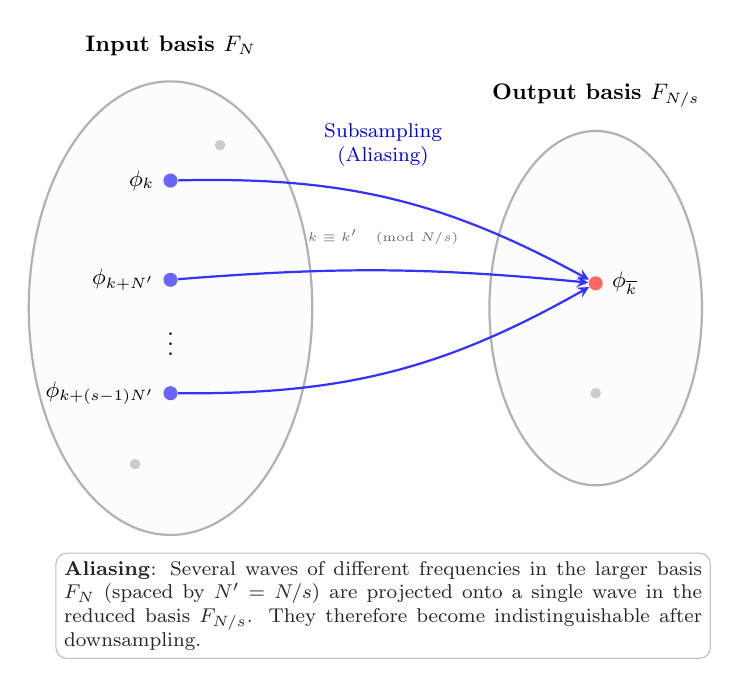
\begin{tikzpicture}[scale=0.9, transform shape]
        % --- ENSEMBLES (Patates) ---
        \draw[thick, gray!60, fill=gray!2] (0,0) ellipse (2cm and 3.2cm);
        \draw[thick, gray!60, fill=gray!2] (6,0) ellipse (1.5cm and 2.5cm);

        % Titres des ensembles
        \node[font=\small\bfseries] at (0, 3.7) {Input basis $F_N$};
        \node[font=\small\bfseries] at (6, 3) {Output basis $F_{N/s}$};

        % --- POINTS/ONDES D'ENTRÉE ---
        % Groupe d'aliasing vers k_bar
        \node[circle, fill=blue!60, inner sep=2pt, label=left:{\small $\phi_k$}] (k1) at (0, 1.8) {};
        \node[circle, fill=blue!60, inner sep=2pt, label=left:{\small $\phi_{k+N'}$}] (k2) at (0, 0.4) {};
        
        % Points de suspension
        \node at (0, -0.4) {$\vdots$};
        
        \node[circle, fill=blue!60, inner sep=2pt, label=left:{\small $\phi_{k+(s-1)N'}$}] (k3) at (0, -1.2) {};
        
        % Autres points pour le style
        \node[circle, fill=gray!40, inner sep=1.5pt] (o1) at (0.7, 2.3) {};
        \node[circle, fill=gray!40, inner sep=1.5pt] (o2) at (-0.5, -2.2) {};

        % --- POINT DE SORTIE ---
        \node[circle, fill=red!60, inner sep=2pt, label=right:{\small $\phi_{\overline{k}}$}] (kout) at (6, 0.35) {};
        
        % Autre point de sortie
        \node[circle, fill=gray!40, inner sep=1.5pt] (oout) at (6, -1.2) {};

        % --- FLÈCHES (PROJECTION) ---
        \draw[->, >=stealth, thick, blue!80, bend left=15] (k1) to (kout);
        \draw[->, >=stealth, thick, blue!80, bend left=5] (k2) to (kout);
        \draw[->, >=stealth, thick, blue!80, bend right=15] (k3) to (kout);

        % Annotations (Positionnement corrigé pour éviter les collisions)
        \node[text=blue!90!black, font=\footnotesize, align=center] at (3, 2.3) {Subsampling \\ (Aliasing)};
        \node[text=black!60, font=\tiny] at (3, 1.0) {$k \equiv k' \pmod{N/s}$};

        % Légende explicative en bas
        \node[draw=gray!50, rounded corners, fill=white, text=black!85, font=\footnotesize, text width=9cm, align=justify] at (3, -4.2) {
            \textbf{Aliasing}: Several waves of different frequencies in the larger basis $F_N$
            (spaced by $N'=N/s$) are projected onto a single wave in the reduced basis $F_{N/s}$.
            They therefore become indistinguishable after downsampling.
        };

    \end{tikzpicture}
    \caption{Set-based representation of generalized spectral folding. The arrows illustrate the loss of injectivity: a set of $s$ source frequencies contributes to a single output frequency.}
    \label{fig:aliasing_mapping}
\end{figure}

\paragraph{Why the previous results no longer apply directly.}

The previous results relied on the fact that circular convolution with stride $1$
preserves spatial size and acts separately on each Fourier frequency. This separation
yields singular vectors associated with a single frequency. Once a layer reduces
spatial resolution, this property disappears: subsampling groups several
input frequencies into the same output frequency. We now formalize this
grouping, or aliasing.

\subsection{Spatial Subsampling and Frequency Aliasing}

To simplify the analysis, we first isolate the effect of subsampling, independently of any convolution.
Assume that $s$ divides $N$, and let
\[
    N' = \frac{N}{s}.
\]
We define the subsampling operator
\[
    P_s : \mathbb{C}^N \longrightarrow \mathbb{C}^{N'}
\]
by
\begin{equation*}
    (P_s x)_r = x_{sr},
    \qquad r = 0,\dots,N'-1.
\end{equation*}
In other words, $P_s$ retains one value every $s$ positions.

Now let $(F_N)_k$ be a 1D Fourier direction of size $N$. Applying $P_s$ to this
direction gives, for every $r=0,\dots,N'-1$,
\begin{align*}
    \big(P_s (F_N)_k\big)_r
    &= ((F_N)_k)_{sr} \notag \\
    &= \frac{1}{\sqrt{N}}
       \exp\left(2\pi i \frac{k sr}{N}\right) \notag \\
    &= \frac{1}{\sqrt{N}}
       \exp\left(2\pi i \frac{k r}{N'}\right).
\end{align*}
The preceding exponential depends on $k$ modulo $N'$. Writing
\[
    \overline{k} = k \bmod N',
\]
and since $N=sN'$, so that
\[
    \frac{1}{\sqrt{N}} = \frac{1}{\sqrt{s}}\frac{1}{\sqrt{N'}},
\]
we obtain
\begin{equation}
    P_s (F_N)_k
    =
    \frac{1}{\sqrt{s}}(F_{N'})_{\overline{k}}.
    \label{eq:sous_echantillonnage_fourier_1d}
\end{equation}

This means that, after subsampling, frequency $k$ at size $N$ becomes frequency $\overline{k}$ at size $N'$.
This equation precisely expresses \textit{aliasing}. Two frequencies $k$ and $k'$
such that
\[
    k \equiv k' \pmod{N'}
\]
become identical after subsampling.
Thus, for each frequency $\overline{k} \in \{0,\dots,N'-1\}$, there is a set of $s$ source frequencies
in the original signal,
\[
    \mathcal{A}_k
    =
    \left\{ \overline{k} + qN' \mid q \in \{0,\dots,s-1\} \right\},
\]
that become indistinguishable after subsampling.

In other words, the subsampling operator is not \textbf{injective} in the frequency domain:
$s$ distinct frequencies in the domain, spaced by $N'$, project onto a single frequency in
the codomain.

\paragraph{Extension to the two-dimensional case.}

We now extend this reasoning to images of size $N \times N$. We define the 2D spatial
subsampling operator
\[
    P_s^{(2D)} : \mathbb{C}^{N \times N} \longrightarrow \mathbb{C}^{N' \times N'}
\]
by
\begin{equation}
    \big(P_s^{(2D)}X\big)_{r,t}
    =
    X_{sr,st},
    \qquad r,t = 0,\dots,N'-1.
    \label{eq:def_sous_echantillonnage_2d}
\end{equation}
It therefore retains one row in $s$ and one column in $s$.

After vectorization, let $\Pi_s$ denote the matrix associated with the operator
$P_s^{(2D)}$. For the vectorized Fourier direction
\[
    q_{u,v}
    =
    (F_N)_v \otimes (F_N)_u,
\]
the 1D result can be applied along each of the two dimensions. Using the
1D result obtained in \eqref{eq:sous_echantillonnage_fourier_1d} along each dimension gives
\begin{align}
    \Pi_s q_{u,v}
    &=
    \Pi_s\big((F_N)_v \otimes (F_N)_u\big) \notag \\
    &=
    \big(P_s(F_N)_v\big) \otimes \big(P_s(F_N)_u\big) \notag \\
    &=
    \left(\frac{1}{\sqrt{s}}(F_{N'})_{\overline{v}}\right)
    \otimes
    \left(\frac{1}{\sqrt{s}}(F_{N'})_{\overline{u}}\right) \notag \\
    &=
    \frac{1}{s}
    (F_{N'})_{\overline{v}} \otimes (F_{N'})_{\overline{u}}.
    \label{eq:sous_echantillonnage_fourier_2d}
\end{align}
Here,
\[
    \overline{u} = u \bmod N',
    \qquad
    \overline{v} = v \bmod N'.
\]

Thus, two 2D frequencies $(u,v)$ and $(u',v')$ become indistinguishable after subsampling
whenever
\[
    u \equiv u' \pmod{N'},
    \qquad
    v \equiv v' \pmod{N'}.
\]
For each output frequency $(\overline{u},\overline{v})$, the set of input frequencies
that project onto it is therefore
\begin{equation}
    \mathcal{A}_{\overline{u},\overline{v}}
    =
    \left\{
        (\overline{u}+q_1N',\,\overline{v}+q_2N')
        \;\middle|\;
        q_1,q_2 \in \{0,\dots,s-1\}
    \right\}.
    \label{eq:classe_aliasing_2d}
\end{equation}

\subsection{Strided Convolution and Spectral Folding}

We now return to a convolutional layer. A convolution with stride $s$ can be viewed
as an ordinary convolution with stride $1$, followed by noncommutative spatial subsampling. After vectorization,
if $M_h$ denotes the operator associated with circular convolution with stride $1$ and kernel $h$, and
$\Pi_s$ denotes the subsampling matrix associated with $P_s^{(2D)}$, the convolution operator
with stride $s$ is
\begin{equation}
    M_h^{(s)}
    =
    \Pi_s M_h.
    \label{eq:conv_stride_sampling}
\end{equation}

This expression means that all convolution values are computed first, and only
positions whose two spatial indices are multiples of $s$ are then retained.

Since $M_h$ is a circular convolution with stride $1$, this direction is an eigendirection of
the operator. Using the diagonalization recalled in \eqref{eq:diagonalisation_conv_2d}, we have
\[
    M_h q_{u,v}
    =
    \lambda_{u,v} q_{u,v},
\]
where $\lambda_{u,v}$ is the eigenvalue associated with frequency $(u,v)$.

Applying subsampling next, and using
\eqref{eq:sous_echantillonnage_fourier_2d}, gives

\begin{align}
    M_h^{(s)} q_{u,v}
    &=
    \Pi_s M_h q_{u,v} \notag \\
    &=
    \lambda_{u,v}\Pi_s q_{u,v} \notag \\
    &=
    \frac{\lambda_{u,v}}{s}
    q_{\overline{u},\overline{v}}^{(N')},
    \label{eq:action_conv_stride_fourier}
\end{align}

where
\[
    q_{\overline{u},\overline{v}}^{(N')}
    =
    (F_{N'})_{\overline{v}} \otimes (F_{N'})_{\overline{u}}.
\]

Here,
\[
    \overline{u}=u \bmod N',
    \qquad
    \overline{v}=v \bmod N'.
\]

Equation~\eqref{eq:action_conv_stride_fourier} shows that strided convolution preserves part
of the Fourier structure, but with an essential difference: several input frequencies can be
mapped to the same output frequency. More precisely, all frequencies belonging to the same
aliasing class
\[
    \mathcal{A}_{\overline{u},\overline{v}}
    =
    \left\{
        (\overline{u}+q_1N',\,\overline{v}+q_2N')
        \;\middle|\;
        q_1,q_2\in\{0,\dots,s-1\}
    \right\}
\]
are associated with the same output frequency $(\overline{u},\overline{v})$.

To express this grouping in matrix form, we introduce the matrix
\[
    \mathcal{S}_s \in \mathbb{C}^{N'^2 \times N^2},
\]
which describes spectral folding in the Fourier basis. Its columns correspond to input
frequencies $(u,v)$ and its rows to output frequencies $(\alpha,\beta)$. We define
\begin{equation}
    (\mathcal{S}_s)_{(\alpha,\beta),(u,v)}
    =
    \begin{cases}
        \dfrac{1}{s},
        & \text{if } \alpha = u \bmod N'
        \text{ and } \beta = v \bmod N', \\[0.4em]
        0,
        & \text{otherwise.}
    \end{cases}
    \label{eq:def_matrice_sampling_fourier}
\end{equation}

Thus, for a given input frequency $(u,v)$, the matrix $\mathcal{S}_s$ places a single nonzero
coefficient in the row corresponding to the output frequency
\[
    (u \bmod N',\, v \bmod N').
\]
This coefficient equals $\frac{1}{s}$, as in \eqref{eq:sous_echantillonnage_fourier_2d}.

The action of subsampling on the entire Fourier basis can then be written as
\begin{equation}
    \Pi_s Q_N
    =
    Q_{N'} \mathcal{S}_s.
    \label{eq:sampling_base_fourier}
\end{equation}
Since $Q_N$ is unitary, we obtain the factorization
\begin{equation}
    \Pi_s
    =
    Q_{N'} \mathcal{S}_s Q_N^H.
    \label{eq:factorisation_sampling_fourier}
\end{equation}

This expression confirms that $\mathcal{S}_s$ represents aliasing in the frequency domain.
Indeed, if
\[
    \widehat{x}=Q_N^H x
\]
denotes the Fourier coefficients of the input, the Fourier coefficients of the subsampled output
are given by
\[
    \widehat{y}
    =
    Q_{N'}^H\Pi_s x
    =
    \mathcal{S}_s \widehat{x}.
\]
By the definition of $\mathcal{S}_s$, this gives, for each output frequency $(\alpha,\beta)$,
\begin{equation}
    \widehat{y}_{\alpha,\beta}
    =
    \frac{1}{s}
    \sum_{(u,v)\in\mathcal{A}_{\alpha,\beta}}
    \widehat{x}_{u,v}.
    \label{eq:somme_coefficients_aliasing}
\end{equation}

In other words, subsampling does not retain the Fourier coefficients separately:
it sums the coefficients belonging to the same aliasing class. This mechanism explains
why, in a strided layer, singular directions are no longer necessarily associated
with a single Fourier frequency.

\subsection{Composition with a Convolution of Stride $1$}

We can now combine subsampling with circular convolution of stride $1$.
Consider a multichannel convolutional layer with stride $1$, represented by the matrix
operator $M$. From the factorization established in \eqref{eq:factorisation_M},
\begin{equation*}
    M
    =
    (I_{m_{\mathrm{out}}} \otimes Q_N)
    L
    (I_{m_{\mathrm{in}}} \otimes Q_N)^H,
\end{equation*}

A convolution with stride $s$ is then obtained by first applying convolution with stride $1$,
and then retaining only one position in $s$ along each spatial direction. Since this reduction
is performed separately on each output channel, we introduce
\[
    \Pi_s^{\mathrm{out}}
    =
    I_{m_{\mathrm{out}}} \otimes \Pi_s.
\]
The operator corresponding to convolution with stride $s$ is then
\begin{equation*}
    M^{(s)}
    =
    \Pi_s^{\mathrm{out}} M.
\end{equation*}

Substituting the Fourier factorization of $M$ and the factorization of $\Pi_s$ obtained in
\eqref{eq:factorisation_sampling_fourier} gives
\begin{align*}
    M^{(s)}
    &=
    (I_{m_{\mathrm{out}}} \otimes \Pi_s)
    (I_{m_{\mathrm{out}}} \otimes Q_N)
    L
    (I_{m_{\mathrm{in}}} \otimes Q_N)^H \notag \\
    &=
    (I_{m_{\mathrm{out}}} \otimes Q_{N'})
    (I_{m_{\mathrm{out}}} \otimes \mathcal{S}_s)
    L
    (I_{m_{\mathrm{in}}} \otimes Q_N)^H.
\end{align*}

This expression makes the difference from the stride-$1$ case clear. The factor $L$
still acts frequency by frequency. The factor $\mathcal{S}_s$, however, subsequently groups
several input frequencies into a single output frequency.

To examine this grouping more closely, we use the same reasoning as above.
Let

\begin{equation*}
    \widehat{x}_{u,v} \in \mathbb{C}^{m_{\mathrm{in}}}
    \qquad \text{and} \qquad
    \widehat{z}_{u,v} = G^{(u,v)} \widehat{x}_{u,v}.
\end{equation*}

We then apply subsampling for a reduced frequency $(\alpha,\beta)$:
\begin{align}
    \widehat{y}_{\alpha,\beta}
    &=
    \frac{1}{s}
    \sum_{(u,v)\in\mathcal{A}_{\alpha,\beta}}
    \widehat{z}_{u,v} \notag \\
    &=
    \frac{1}{s}
    \sum_{(u,v)\in\mathcal{A}_{\alpha,\beta}}
    G^{(u,v)}\widehat{x}_{u,v}.
    \label{eq:sortie_stride_classe_aliasing}
\end{align}

To express this relation in matrix form, we fix an arbitrary ordering of the frequencies in
the aliasing class:
\[
    \mathcal{A}_{\alpha,\beta}
    =
    \{(u_1,v_1),\dots,(u_{s^2},v_{s^2})\}.
\]
We then collect the corresponding input coefficients in a single vector:
\[
    \widehat{x}_{\mathcal{A}_{\alpha,\beta}}
    =
    \begin{pmatrix}
        \widehat{x}_{u_1,v_1} \\
        \vdots \\
        \widehat{x}_{u_{s^2},v_{s^2}}
    \end{pmatrix}
    \in \mathbb{C}^{m_{\mathrm{in}}s^2}.
\]

This gives the matrix
\begin{equation}
    G_s^{(\alpha,\beta)}
    =
    \frac{1}{s}
    \begin{pmatrix}
        G^{(u_1,v_1)}
        &
        G^{(u_2,v_2)}
        &
        \cdots
        &
        G^{(u_{s^2},v_{s^2})}
    \end{pmatrix}
    \in
    \mathbb{C}^{m_{\mathrm{out}}\times m_{\mathrm{in}}s^2}.
    \label{eq:def_matrice_aliasing_stride}
\end{equation}

This matrix is simply a compact way to express the sum in
\eqref{eq:sortie_stride_classe_aliasing}. Multiplying
$G_s^{(\alpha,\beta)}$ by the stacked vector
$\widehat{x}_{\mathcal{A}_{\alpha,\beta}}$ gives exactly
\[
    \frac{1}{s}
    \sum_{(u,v)\in\mathcal{A}_{\alpha,\beta}}
    G^{(u,v)}\widehat{x}_{u,v}.
\]
By construction, therefore,
\begin{equation*}
    \widehat{y}_{\alpha,\beta}
    =
    G_s^{(\alpha,\beta)}
    \widehat{x}_{\mathcal{A}_{\alpha,\beta}}.
\end{equation*}

This formulation reduces the study of the structural sensitivity of a convolution with stride $s$ to
a local analysis, one output frequency at a time. For each reduced frequency $(\alpha,\beta)$,
we therefore study the singular values and vectors of the matrix $G_s^{(\alpha,\beta)}$.

\subsection{Construction of Right Singular Vectors}

\begin{proof}

To simplify the notation, let
\[
    \varphi_{u,v}^{(N)}
    =
    (F_N)_v \otimes (F_N)_u,
    \qquad
    \varphi_{\alpha,\beta}^{(N')}
    =
    (F_{N'})_\beta \otimes (F_{N'})_\alpha.
\]

Fix an output frequency $(\alpha,\beta)$ and its aliasing class
$\mathcal{A}_{\alpha,\beta}$. Choosing an arbitrary ordering of this class,
we write
\[
    \mathcal{A}_{\alpha,\beta}
    =
    \{(u_1,v_1),\dots,(u_{s^2},v_{s^2})\}.
\]
Let
\[
    p
    =
    \begin{pmatrix}
        p_{u_1,v_1} \\
        \vdots \\
        p_{u_{s^2},v_{s^2}}
    \end{pmatrix}
    \in \mathbb{C}^{m_{\mathrm{in}}s^2},
    \qquad
    p_{u_i,v_i}\in\mathbb{C}^{m_{\mathrm{in}}},
\]
be a right singular vector of $G_s^{(\alpha,\beta)}$, associated with a singular value
$\sigma$ and a left singular vector $q\in\mathbb{C}^{m_{\mathrm{out}}}$. We therefore have
\begin{equation}
    G_s^{(\alpha,\beta)}p
    =
    \sigma q,
    \qquad
    G_s^{(\alpha,\beta)H}q
    =
    \sigma p.
    \label{eq:svd_matrice_aliasing_stride}
\end{equation}

From the blocks $p_{u,v}$, we construct the input vector
\begin{equation}
    r
    =
    \sum_{(u,v)\in\mathcal{A}_{\alpha,\beta}}
    p_{u,v}\otimes \varphi_{u,v}^{(N)}.
    \label{eq:construction_vecteur_singulier_stride}
\end{equation}
This vector is therefore no longer associated with a single Fourier frequency: it is a combination
of all frequencies belonging to the same aliasing class.

We now show that $r$ is a right singular vector of $M^{(s)}$. By
\eqref{eq:sortie_stride_classe_aliasing}, the action of $M^{(s)}$ on the Fourier coefficients
associated with the class $\mathcal{A}_{\alpha,\beta}$ is given by
\[
    \widehat{y}_{\alpha,\beta}
    =
    \frac{1}{s}
    \sum_{(u,v)\in\mathcal{A}_{\alpha,\beta}}
    G^{(u,v)}p_{u,v}.
\]
By the definition of $G_s^{(\alpha,\beta)}$, this sum is simply
\[
    \widehat{y}_{\alpha,\beta}
    =
    G_s^{(\alpha,\beta)}p.
\]
Using the singular-vector relation \eqref{eq:svd_matrice_aliasing_stride}, we therefore obtain
\[
    \widehat{y}_{\alpha,\beta}
    =
    \sigma q.
\]
In the spatial domain, this gives
\[
    M^{(s)}r
    =
    \sigma q\otimes \varphi_{\alpha,\beta}^{(N')}.
\]
Defining
\[
    w
    =
    q\otimes \varphi_{\alpha,\beta}^{(N')},
\]
gives
\begin{equation}
    M^{(s)}r = \sigma w.
    \label{eq:relation_singuliere_stride_droite}
\end{equation}

It remains to verify the adjoint equation. The adjoint of $M^{(s)}$ maps an output frequency
$(\alpha,\beta)$ back to all input frequencies in the class
$\mathcal{A}_{\alpha,\beta}$. This gives
\[
    M^{(s)H}w
    =
    \sum_{(u,v)\in\mathcal{A}_{\alpha,\beta}}
    \frac{1}{s}
    \left(
        G^{(u,v)H}q
    \right)
    \otimes
    \varphi_{u,v}^{(N)}.
\]
The relation
\[
    G_s^{(\alpha,\beta)H}q=\sigma p
\]
implies, block by block, that
\[
    \frac{1}{s}G^{(u,v)H}q
    =
    \sigma p_{u,v},
    \qquad
    (u,v)\in\mathcal{A}_{\alpha,\beta}.
\]
Substituting into the preceding expression gives directly
\begin{equation}
    M^{(s)H}w
    =
    \sigma r.
    \label{eq:relation_singuliere_stride_gauche}
\end{equation}

The two relations
\[
    M^{(s)}r=\sigma w,
    \qquad
    M^{(s)H}w=\sigma r
\]
therefore show that $r$ and $w$ form a pair of right and left singular vectors
of $M^{(s)}$.

Finally, normalization is preserved. The frequencies in
$\mathcal{A}_{\alpha,\beta}$ are distinct, so the corresponding directions
$\varphi_{u,v}^{(N)}$ are orthonormal. Thus,
\[
    \|r\|_2^2
    =
    \sum_{(u,v)\in\mathcal{A}_{\alpha,\beta}}
    \|p_{u,v}\|_2^2
    =
    \|p\|_2^2.
\]
If $p$ is normalized, then $r$ is also normalized. Similarly, if $q$ is normalized,
then $w=q\otimes \varphi_{\alpha,\beta}^{(N')}$ is normalized.

This recovers the result stated in Proposition~5 of Tsuzuku and Sato
\cite{tsuzuku2019structural}: in a downsampling layer, singular directions
are no longer necessarily pure Fourier directions. They can be combinations
of frequencies belonging to the same aliasing class.

\end{proof}

\subsection{Average Pooling as a Special Case}

\textit{Average pooling} replaces each local window of size $s\times s$
with the average of its pixels, as illustrated in Figure~\ref{fig:avg_pooling_spatial}. This operation therefore reduces spatial resolution, like a
strided convolution. The difference is that a fixed averaging filter is applied
before subsampling.

In the circular setting used here, this filter can be represented by the kernel
\[
    h_{\mathrm{avg}}[a,b]
    =
    \begin{cases}
        \dfrac{1}{s^2},
        & \text{if } a,b \in \{0,\dots,s-1\},\\[0.4em]
        0,
        & \text{otherwise,}
    \end{cases}
\]
where spatial indices are interpreted modulo $N$. Convolution with
$h_{\mathrm{avg}}$ therefore computes a local average, after which subsampling retains
one position in $s$ along each spatial direction.

In the multichannel case, this operation is applied separately to each channel. If $m$
denotes the number of channels and
$C_{h_{\mathrm{avg}}}\in\mathbb{C}^{N^2\times N^2}$ denotes the circular convolution matrix
associated with the averaging kernel, the \textit{average pooling} operator is
\begin{equation}
    M_{\mathrm{avg}}^{(s)}
    =
    (I_m \otimes \Pi_s)
    (I_m \otimes C_{h_{\mathrm{avg}}}).
    \label{eq:average_pooling_convolution_sampling}
\end{equation}

This is exactly the case studied previously: circular convolution with stride $1$,
followed by subsampling. The averaging kernel acts as a low-pass filter, attenuating
certain frequencies before spectral folding. However, the aliasing mechanism remains the same:
several input frequencies can be grouped into a single output frequency.

Consequently, the right singular vectors of an \textit{average pooling} layer can also
be chosen as combinations of frequencies belonging to the same aliasing class.

\section{Real-Valued Image Constraint}
\label{sec:contrainte-image-reelle}

Proposition~6 of Tsuzuku and Sato~\cite{tsuzuku2019structural} addresses the problem of applying
the methods just developed to practical cases. Images processed by a network are real-valued,
whereas an individual Fourier function is generally complex. The idea is to show that the requirement
that an image be real-valued can be met using the Hermitian symmetry of its Fourier coefficients. To this end, we
introduce the tools needed to understand this symmetry.

We begin with the 2D discrete Fourier transform~\cite{ImagerieNumeriqueTheme7Block2}. For an image
$X\in\mathbb{C}^{N\times N}$, we define
\begin{equation*}
    \widehat{X}_{u,v}
    =
    S(X)_{u,v}
    =
    \sum_{m=0}^{N-1}\sum_{n=0}^{N-1}
    X[m,n]\,
    \exp\left(
        -2\pi i\frac{um+vn}{N}
    \right),
    \qquad
    u,v\in\{0,\dots,N-1\}.
\end{equation*}

The image can be reconstructed from its Fourier coefficients using the inverse transform:
\begin{equation}
    X[m,n]
    =
    \frac{1}{N^2}
    \sum_{u=0}^{N-1}\sum_{v=0}^{N-1}
    \widehat{X}_{u,v}\,
    \exp\left(
        2\pi i\frac{um+vn}{N}
    \right).
    \label{eq:idft2d_definition}
\end{equation}

These formulas are compatible with the Fourier bases introduced previously, up to a
normalization factor. Here, we follow the notation $S(X)$ used in the paper \cite{tsuzuku2019structural} to reproduce
Proposition~6 directly.

\subsection{Hermitian Symmetry of Fourier Coefficients}

The requirement that an image be real-valued corresponds to a particular symmetry of its Fourier
coefficients. More precisely, for an image $X\in\mathbb{C}^{N\times N}$,
\begin{equation}
    X\in\mathbb{R}^{N\times N}
    \quad\Longleftrightarrow\quad
    \widehat{X}_{u,v}
    =
    \widehat{X}^{*}_{(-u)\bmod N,\,(-v)\bmod N},
    \qquad
    u,v\in\{0,\dots,N-1\}.
    \label{eq:symetrie_hermitienne_fourier}
\end{equation}
This property is the Hermitian symmetry of the Fourier transform of a real-valued signal. It is
a standard result in discrete signal processing~\cite{oppenheim2009discrete}, and here corresponds to
Proposition~6 of Tsuzuku and Sato~\cite{tsuzuku2019structural}.

We first prove the forward implication. Assume that $X$ is real-valued, that is,
\[
    X[m,n]^* = X[m,n]
    \qquad
    \text{for all } m,n.
\]
By the definition of the 2D DFT,
\begin{align*}
    \widehat{X}^{*}_{u,v}
    &=
    \left(
        \sum_{m=0}^{N-1}\sum_{n=0}^{N-1}
        X[m,n]\,
        \exp\left(-2\pi i\frac{um+vn}{N}\right)
    \right)^* \notag \\
    &=
    \sum_{m=0}^{N-1}\sum_{n=0}^{N-1}
    X[m,n]^*\,
    \exp\left(2\pi i\frac{um+vn}{N}\right) \notag \\
    &=
    \sum_{m=0}^{N-1}\sum_{n=0}^{N-1}
    X[m,n]\,
    \exp\left(-2\pi i\frac{((-u)m+(-v)n)}{N}\right) \notag \\
    &=
    \widehat{X}_{(-u)\bmod N,\,(-v)\bmod N}.
\end{align*}
We therefore obtain
\[
    \widehat{X}_{u,v}
    =
    \widehat{X}^{*}_{(-u)\bmod N,\,(-v)\bmod N}.
\]

We now prove the converse. Suppose the Fourier coefficients satisfy the symmetry
\eqref{eq:symetrie_hermitienne_fourier}. We want to show that the reconstructed image is real-valued.
Starting from the inverse Fourier transform \eqref{eq:idft2d_definition}, we compute the conjugate
of $X[m,n]$:
\begin{align*}
    X[m,n]^*
    &=
    \left(
        \frac{1}{N^2}
        \sum_{u=0}^{N-1}\sum_{v=0}^{N-1}
        \widehat{X}_{u,v}
        \exp\left(2\pi i\frac{um+vn}{N}\right)
    \right)^* \notag \\
    &=
    \frac{1}{N^2}
    \sum_{u=0}^{N-1}\sum_{v=0}^{N-1}
    \widehat{X}^{*}_{u,v}
    \exp\left(-2\pi i\frac{um+vn}{N}\right).
\end{align*}
Recall that the Hermitian symmetry assumption gives
\[
    \widehat{X}^{*}_{u,v}
    =
    \widehat{X}_{(-u)\bmod N,\,(-v)\bmod N}.
\]
Therefore,
\begin{align*}
    X[m,n]^*
    &=
    \frac{1}{N^2}
    \sum_{u=0}^{N-1}\sum_{v=0}^{N-1}
    \widehat{X}_{(-u)\bmod N,\,(-v)\bmod N}
    \exp\left(-2\pi i\frac{um+vn}{N}\right).
\end{align*}
Changing indices according to
\[
    u' = (-u)\bmod N,
    \qquad
    v' = (-v)\bmod N,
\]
gives
\begin{align*}
    X[m,n]^*
    &=
    \frac{1}{N^2}
    \sum_{u'=0}^{N-1}\sum_{v'=0}^{N-1}
    \widehat{X}_{u',v'}
    \exp\left(2\pi i\frac{u'm+v'n}{N}\right) \notag \\
    &=
    X[m,n].
\end{align*}
Thus, $X[m,n]^*=X[m,n]$ for all $m,n$, so $X$ is real-valued.

We have therefore established the equivalence:
\[
    X\in\mathbb{R}^{N\times N}
    \quad\Longleftrightarrow\quad
    \widehat{X}_{u,v}
    =
    \widehat{X}^{*}_{(-u)\bmod N,\,(-v)\bmod N}.
\]

\subsection{Consequence for Fourier Perturbations}

The preceding equivalence applies directly to the perturbations we wish to add to images.
Since the images processed by the network are real-valued,
\[
    x \in \mathbb{R}^{N\times N\times c},
\]
an admissible perturbation must also be real-valued in the spatial domain. Thus, for each channel,
its Fourier coefficients must satisfy Hermitian symmetry:
\begin{equation}
    \widehat{\delta}_{(-u)\bmod N,\,(-v)\bmod N}
    =
    \widehat{\delta}_{u,v}^{*}.
    \label{eq:contrainte_reelle_perturbation_fourier}
\end{equation}

In other words, if a frequency \((u,v)\) is used, its opposite frequency
\[
    ((-u)\bmod N,\,(-v)\bmod N)
\]
must also be used with the conjugate coefficient. This condition guarantees that the inverse Fourier transform yields a real-valued perturbation.

There are a few special cases in which a frequency equals its own opposite modulo $N$.
These frequencies satisfy
\[
    (u,v)
    =
    ((-u)\bmod N,\,(-v)\bmod N).
\]
In this case, the preceding condition simply requires the Fourier coefficient to be real. For
even $N$, this applies in particular to the frequencies
\[
    (0,0),
    \qquad
    (N/2,0),
    \qquad
    (0,N/2),
    \qquad
    (N/2,N/2).
\]
Outside these special cases, frequencies must be taken in conjugate pairs.

Tsuzuku and Sato use this idea in their \textit{Single Fourier Attack}
\cite{tsuzuku2019structural}. 
For a non-self-conjugate frequency, a \textit{Single Fourier Attack} perturbation
can then be written as
\begin{equation}
    \delta_{u,v}
    =
    \eta
    \left[
        (1+i)\,q_{u,v}
        +
        (1-i)\,q_{(-u)\bmod N,\,(-v)\bmod N}
    \right].
    \label{eq:sfa_perturbation_fourier}
\end{equation}

The coefficients $(1+i)$ and $(1-i)$ are conjugates of one another, and the two Fourier directions
correspond to opposite frequencies. The perturbation therefore satisfies condition
\eqref{eq:contrainte_reelle_perturbation_fourier}, guaranteeing that it is real-valued in the spatial domain.

The parameter $\eta$ controls the perturbation amplitude in this theoretical expression. In practice,
adversarial experiments instead impose a bound on the pixels, for example,
\[
    \|\delta\|_\infty \leq \varepsilon.
\]

\section{Limitations and Scope of the Theoretical Framework}

The preceding results provide a clear mathematical explanation for the special role
of Fourier directions in convolutional networks. However, the exact scope
of this result must be specified.

\subsection{An Exact Result in a Controlled Setting}

The preceding reasoning is exact in a specific setting: circular convolutions, linear
layers, and sensitivity analysis using singular values. Under these assumptions, the
factorization in \eqref{eq:factorisation_M} allows the network to be studied frequency by
frequency. The resulting singular directions then have the form
\[
    a \otimes q_{u,v},
\]
where $q_{u,v}$ describes the spatial Fourier pattern and $a$ the channel mixing.

This result should therefore be understood as a structural property of convolutions, rather than
a complete description of an actual CNN.

\subsection{Differences from Practical Architectures}

Architectures used in practice depart from this exact setting. \textit{Zero-padding}
often replaces circular padding, preventing exact diagonalization by the Fourier
basis. Downsampling layers, such as strided convolutions and \textit{average
pooling}, introduce aliasing, as already discussed in
Section~\ref{sec:couches-reduction-stride-pooling}.

Finally, ReLU activations and \textit{max-pooling} make the network nonlinear. The complete
network can therefore no longer be viewed as a single linear operator diagonalizable in the Fourier basis.
However, these operations have a piecewise linear structure, allowing
a local interpretation of frequency analysis to be retained.

\subsection{Local Scope of Frequency Analysis in Nonlinear CNNs}

In this subsection, $f$ denotes the mapping performed by the network
up to the logits, before the final \textit{argmax} operation, which is not an affine map.

Networks using piecewise linear activations, such as ReLU, can be viewed
as piecewise affine functions: input space is divided into regions, and on
each region the network performs an affine map~\cite{montufar2014number,balestriero2018spline}.
This observation clarifies the scope of frequency analysis in practical CNNs:
the complete network is not globally linear, but its behavior can be described
locally by an affine map as long as the activation and pooling choices remain fixed.

This leads me to the following proposition:

\begin{proposition}[Local Linearization of a CNN with ReLU and Max-Pooling]
Let $f$ be a convolutional network consisting of convolutional layers, ReLU activations, and
max-pooling layers. For any input $x$ that does not lie
on a boundary between linear regions, that is, when the ReLU
pre-activations have nonzero signs and the selected maxima in the pooling windows
are unique, there exists a neighborhood $\mathcal{V}_x$ of $x$ such that, for every
$z \in \mathcal{V}_x$,
\[
    f(z) = A_x z + b_x,
\]
where $A_x$ is a matrix depending on the linear region containing $x$.
\end{proposition}

\begin{proof}
A ReLU activation acts coordinate by coordinate according to
\[
    \mathrm{ReLU}(t)=\max(t,0).
\]
Consider a given layer of the network, and let $a_\ell$ denote its pre-activation vector.
If the sign of each coordinate of $a_\ell$ is fixed in a neighborhood of $x$, then ReLU
acts as a linear map on this region:
\[
    \mathrm{ReLU}(a_\ell)=D_\ell(x)a_\ell,
\]
where $D_\ell(x)$ is a diagonal matrix whose entries are $0$ or $1$ depending on whether the
corresponding coordinates are inactive or active.

Similarly, a max-pooling layer selects the coordinate with the largest value
in each local window. When this maximum is unique in every window, the selected indices
remain unchanged in a sufficiently small neighborhood of $x$. In this region, max-pooling
therefore becomes a linear selection map:
\[
    \mathrm{MaxPool}(z)=P_\ell(x)z,
\]
where $P_\ell(x)$ is a selection matrix depending on the region under consideration. This matrix
encodes both the selection of local maxima and the spatial reduction induced by pooling.

Thus, as long as we remain in a region where the ReLU signs and the indices selected
by max-pooling do not change, every network operation is affine or linear. The
composition of these operations is therefore itself affine. There consequently exist a matrix $A_x$ and a
vector $b_x$ such that
\[
    f(z)=A_xz+b_x.
\]

This local region can be understood as the set of inputs for which the ReLU activation
masks and the indices selected by the max-pooling layers remain unchanged.
\footnote{A more detailed study could explicitly define this region,
for example as the set of points (z) with the same ReLU pre-activation
signs and indices of maxima in the pooling windows as the input (x).
Analyzing the size of this region would provide a more precise measure of the local
validity of the linearization, but lies beyond the scope of this work.}

\end{proof}

This proposition shows that a CNN consisting of convolutions, ReLU, and max-pooling is
piecewise affine. Around an input $x$, as long as the perturbation changes neither the activation masks nor the positions selected
by pooling, the network's behavior is exactly linear up to a bias. Thus, for
every $x+\delta\in\mathcal{V}_x$,
\[
    f(x+\delta)-f(x)=J_f(x)\delta.
\]

In such a region, the Jacobian can be viewed as a product of matrices associated with
the different network operations. For example, in the schematic case of a stack of
convolution--ReLU--pooling blocks, we can write
\[
    J_f(x)
    =
    W_L P_{L-1}(x)D_{L-1}(x)M_{L-1}
    \cdots
    P_1(x)D_1(x)M_1,
\]
where the matrices $M_\ell$ represent convolutions, the matrices $D_\ell(x)$ the ReLU
masks, the matrices $P_\ell(x)$ the selections induced by max-pooling, and $W_L$ the final
linear part.

The matrices $D_\ell(x)$ and $P_\ell(x)$ depend on the input. In general, they therefore prevent
global diagonalization of the network in the Fourier basis. A Fourier direction is
no longer an exact eigenvector of the complete mapping.

However, the convolution operators $M_\ell$ remain present in the Jacobian
product. Frequency analysis therefore retains a local scope: it no longer describes
the global network exactly, but it can still explain why certain frequencies are more strongly
amplified than others around particular inputs.

The \textit{Single Fourier Attack} can then be interpreted as empirically exploiting
this local sensitivity. This interpretation extends the linearity hypothesis of Goodfellow et
al.~\cite{goodfellow2015explaining}.

\subsection{Actual Scope of the Result}

The theoretical framework does not predict exactly which frequencies will be most
sensitive for a given architecture. This sensitivity also depends on the learned weights, the
dataset, padding, normalization, nonlinearities, and downsampling layers.

The analysis does, however, explain why Fourier directions are natural
candidates: they arise directly in the linear study of convolutions. Even in a
nonlinear CNN, this structure may remain partially visible through the model's local
Jacobian. The experiments will therefore assess the extent to which this intuition remains
observable in practice.

% \section{Lien avec les perturbations adversariales universelles}

% Le chapitre de contexte a introduit les perturbations adversariales universelles comme des
% perturbations capables d'affecter plusieurs images différentes. Le cadre théorique développé ici
% donne une explication possible à ce phénomène dans le cas des réseaux convolutionnels.

% Dans le modèle linéaire idéalisé, certaines directions de Fourier peuvent être fortement
% amplifiées par les couches convolutionnelles. Une perturbation construite sur une telle fréquence
% peut donc exploiter une sensibilité liée à la structure du réseau plutôt qu'à une image particulière.

% C'est cette idée qui motive la \textit{Single Fourier Attack} de Tsuzuku et
% Sato~\cite{tsuzuku2019structural}. Au lieu de chercher une perturbation libre dans tout l'espace
% des pixels, l'attaque restreint la recherche à une fréquence de Fourier. Dans un CNN réel, cette
% sensibilité n'est plus une propriété exacte globale, mais elle peut rester visible localement et en
% moyenne sur les images.

% La suite du travail consiste donc à construire des cartes de sensibilité fréquentielle afin
% d'observer quelles fréquences affectent réellement le modèle étudié.
